\documentclass[a4paper, gray]{beamer}

\usepackage{times}

\usepackage{verbatim}
\usepackage{color}
\usepackage{listings}

\usepackage{xcolor}
\definecolor{ocre}{RGB}{243,102,25}

\usepackage[german]{babel}
\usepackage[utf8]{inputenc}
\usepackage[T1]{fontenc}

\usepackage{multicol}

%\usepackage{exercise}

\usepackage{graphicx}

\usetheme{default}

%\usepackage{pgfpages}
%\pgfpagesuselayout{resize to}[a4paper,landscape]

\logo{\pgfimage[width=2cm,height=1cm]{img/hfictlogo}}

\definecolor{lbcolor}{rgb}{0.92,0.92,0.92}
\definecolor{cmtcolor}{rgb}{0.0,0.5,0.0}
\lstset{numbers=left,
        numberstyle=\tiny,
        keywordstyle=\color{blue}\bfseries\sffamily,
        identifierstyle=\ttfamily,
        commentstyle=\em,
        stringstyle=\ttfamily,
        extendedchars=true,
        showstringspaces=false,
        language=c++,
        backgroundcolor=\color{lbcolor},
        commentstyle=\color{cmtcolor}}

\RequirePackage[framemethod=default]{mdframed}

% Exercise box	  
\newmdenv[skipabove=7pt,
skipbelow=7pt,
rightline=false,
leftline=true,
topline=false,
bottomline=false,
backgroundcolor=ocre!10,
linecolor=ocre,
innerleftmargin=5pt,
innerrightmargin=5pt,
innertopmargin=5pt,
innerbottommargin=5pt,
leftmargin=0cm,
rightmargin=0cm,
linewidth=4pt]{eBox}

% Theorem box
\newmdenv[skipabove=7pt,
skipbelow=7pt,
backgroundcolor=black!5,
linecolor=ocre,
innerleftmargin=5pt,
innerrightmargin=5pt,
innertopmargin=5pt,
leftmargin=0cm,
rightmargin=0cm,
innerbottommargin=5pt]{tBox}



\newcounter{dummy} 
\numberwithin{dummy}{section}

\newtheorem{exerciseT}{Exercise}[section]
%\newtheorem{theoremeT}[dummy]{Theorem}
%\newtheorem{exampleT}{Example}[section]

\newenvironment{exercise}{\begin{eBox}}{\hfill{\color{ocre}\tiny\ensuremath{\blacksquare}}\end{eBox}}
%\newenvironment{exercise}{\begin{eBox}\begin{exerciseT}}{\hfill{\color{ocre}\tiny\ensuremath{\blacksquare}}\end{exerciseT}\end{eBox}}
%\newenvironment{theorem}{\begin{tBox}\begin{theoremeT}}{\end{theoremeT}\end{tBox}}
%\newenvironment{example}{\begin{exampleT}}{\hfill{\tiny\ensuremath{\blacksquare}}\end{exampleT}}


\title{Object Oriented Programming with C++}
\subtitle{OOP - HF-ICT}
\author{Dave Herzig}
%\institute{scifortek.com}
\date{\today}

\begin{document}

\frame{\titlepage}

\setcounter{tocdepth}{1}

\frame
{
	\frametitle{Agenda}
	\small {\tableofcontents}
}

\section{Basics}

\begin{frame}[fragile]
  \frametitle{C++ Compiler}
  \begin{center}
  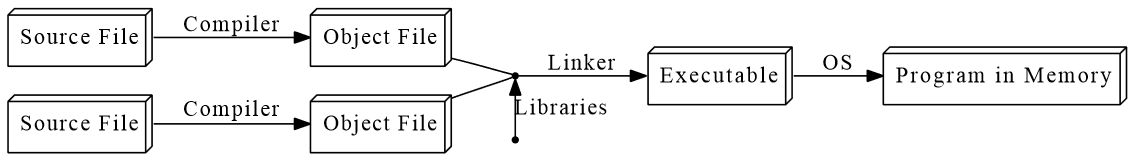
\includegraphics[scale=0.35]{img/compiler.png}
  \end{center}
  \vspace{1mm}
  Commands (GNU C++ Compiler):
  \begin{itemize}
  \item \verb|g++ source.cpp|\\
  {\tiny Compiles and links the source file. An executable file \verb|a.exe| (Windows) or \verb|a.out|
  (Linux) will be created.}
  \item \verb|g++ -c source.cpp|\\
  {\tiny Compiles the source file. An object file \verb|source.o| will be created.}
  \item \verb|g++ -o file.exe source.cpp|\\
  {\tiny Compiles and links the source file. An executable file \verb|file.exe| will be created.}
  \item \verb|g++ -std=c++14 source.cpp|\\
  {\tiny Compiles and links the source file by using the C++ 2014 standard.}
  \end{itemize}
\end{frame}

\begin{frame}[fragile]
  \frametitle{Hello World}
  A Hello World program is a computer program that outputs \verb|"Hello, World!"|. Because this is
  typically the simplest program in most programming languages.
  {\tiny
  \lstinputlisting{code/hello.cpp}
  }
\end{frame}

\begin{frame}[fragile]
  \frametitle{Variables, Datatypes}
  Declaration:
  {\small
\begin{lstlisting}
int n; // one variable with the name n
int a, b; // two variables

// variable with c-like initialization
float x = 5;

// variable with constructor initialization
float y(0);

// variable with uniform initialization (C++ 2011)
float z{0};
\end{lstlisting}
  }
  {\bf A variable will not be initialized!}
\end{frame}

\begin{frame}[fragile]
  \frametitle{Variables, Datatypes}
  Declaration:
  {\small
\begin{lstlisting}
double myNumber;

// var will be an integer, same as a (C++ 2011)
int a = 10;
auto var = a;

// constant. variable which cannot be changed
const int v = 10;
\end{lstlisting}
}
  {\bf A variable will not be initialized!}
\end{frame}

\begin{frame}[fragile]
  \frametitle{Variables, Datatypes}
  {\scriptsize
  \begin{tabular}{|l|l|l|}
  \hline
  \emph{Datatype} & \emph{Number of Bytes} & \emph{Values} \\
  \hline
  \verb|char| & 1 & single character\\
  \verb|int| & 4 & numerical integer type\\
  \verb|long int| & 4 & numerical integer type\\
  \verb|long long int| & 8 & numerical integer type\\
  \verb|short int| & 2 & numerical integer type\\
  \verb|float| & 4 & floating point type\\
  \verb|double| & 8 & floating point type\\
  \verb|bool| & 1 & boolean type \verb|true| or \verb|false|\\
  \hline
  \end{tabular}
  }
  \par
  The number of used bytes is dependent on the compiler and the operating system!
\end{frame}

\begin{frame}[fragile]
  \frametitle{Variables, Datatypes}
  {\scriptsize
  \begin{tabular}{|l|l|l|}
  \hline
  \emph{Datatype} & \emph{Number of Bytes} & \emph{Values} \\
  \hline
  \verb|unsigned char| & 1 & single character\\
  \verb|unsigned int| & 4 & numerical integer type\\
  \verb|unsigend long int| & 4 & numerical integer type\\
  \verb|unsigend long long int| & 8 & numerical integer type\\
  \verb|unsigend short int| & 2 & numerical integer type\\
  \hline
  \end{tabular}
  }
  \par
  The number of used bytes is dependent on the compiler and the operating system!
\end{frame}

\begin{frame}[fragile]
  \frametitle{Variables, Datatypes - Exercise}
  \begin{exercise}
  Write a program which prints out the number of used bytes for each datatype.
  \end{exercise}
\end{frame}

\begin{frame}[fragile]
  \frametitle{Variables, Datatypes - Exercise}
  \begin{exercise}
  A bool variable needs 1 Byte in memory. 1 Byte are 8 Bits. Why does a bool
  variable needs 8 Bits? As there are only two states (\verb|true| and \verb|false|) one Bit
  should be sufficient.
  \end{exercise}
\end{frame}

\begin{frame}[fragile]
	\frametitle{C++ Operators - Assignment}
	The assignment operator \verb|=| assigns a value to a variable.

	\vspace{3mm}

\begin{lstlisting}
a = 5;
\end{lstlisting}
\end{frame}

\begin{frame}[fragile]
	\frametitle{C++ Operators - Arithmetic}
	\begin{itemize}
	\item \verb|+  | Addition
	\item \verb|-  | Subtraction
	\item \verb|*  | Multiplication
	\item \verb|/  | Division
	\item \verb|%  | Modulo
	\item \verb|+= | \verb|i+=7| identical with \verb|i=i+7|
	\item \verb|-= | \verb|i-=7| identical with \verb|i=i-7|
	\item \verb|*= | \verb|i*=7| identical with \verb|i=i*7|
	\item \verb|/= | \verb|i/=7| identical with \verb|i=i/7|
	\item \verb|%= | \verb|i%=7| identical with \verb|i=i%7|
	\end{itemize}
\end{frame}

\begin{frame}[fragile]
	\frametitle{C++ Operators - Increment/Decrement}
	The increase operator \verb|++| and the decrease operator \verb|--| increase or
reduce by one the value stored in a variable.

	\vspace{5mm}

	\verb|i++  | is identical with \verb|i = i + 1|\\
	\verb|i--  | is identical with \verb|i = i - 1|
\end{frame}

\begin{frame}[fragile]
	\frametitle{C++ Operators - Relational}
	Two expressions can be compared using relational and equality operators.
	\begin{itemize}
	\item \verb|== | Equal to
	\item \verb|!= | Not equal to
	\item \verb|>  | Greater than
	\item \verb|<  | Less than
	\item \verb|>= | Greater than or equal to
	\item \verb|<= | Less than or equal to
	\end{itemize}
\end{frame}

\begin{frame}[fragile]
	\frametitle{C++ Operators - Logical}
	The following logical operators are available:

	\begin{itemize}
	\item \verb|!           Not|
	\item \verb|&&          And|
	\item \begin{verbatim}||          Or\end{verbatim}
	\end{itemize}
\end{frame}

\begin{frame}[fragile]
  \frametitle{C++ Operators - Exercise}
  \begin{exercise}
  What is the content of variable \verb|r|?
\begin{lstlisting}
int a = 5, b = 6, c = 7;
bool d = true, e = false;
bool r = (a == b || d) && (c >= 7 && !e);
\end{lstlisting}
  \end{exercise}
\end{frame}

\begin{frame}[fragile]
  \frametitle{Input,Output}
  Streams available in the standard library:
  \begin{itemize}
  \item cin (standard input stream)
  \item cout (standard output stream)
  \item cerr (standard error stream)
  \item clog (standard logging stream)
  \end{itemize}
\end{frame}

\begin{frame}[fragile]
  \frametitle{Input,Output}
  In most program environments, the standard output by default is the screen,
  and the C++ stream object defined to access it is cout.
  {\scriptsize
\begin{lstlisting}
cout << "some text..."; // prints some text... on the screen
cout << 23; // prints the number 23 on the screen
cout << x; // prints the value of x on the screen
cout << "x = " << x << endl; // multiple insertions
\end{lstlisting}
  }
\end{frame}

\begin{frame}[fragile]
  \frametitle{Input,Output}
  In most program environments, the standard input by default is the keyboard,
  and the C++ stream object defined to access it is cin.
\begin{lstlisting}
int number;
cin >> number;
\end{lstlisting}
\end{frame}

\begin{frame}[fragile]
  \frametitle{Input,Output - Exercise}
  \begin{exercise}
  Write a program which reads the height of a satellite and prints out
  the time used for one rotation of the earth.\\
  The formulae to calculate the time is
  \begin{displaymath}
T[sec] = \frac{2 \cdot \pi}{R_{E}} \cdot \sqrt{\frac{(R_{E}+h)^{3}}{g}}
\end{displaymath}

$g$ is the acceleration of gravity: $g = 9.80665 m/s^{2}$\\
$R_{E}$ radius of the earth: $R_{E} = 6371 km$\\
$\pi = 3.14159$\\
  \end{exercise}
\end{frame}

\begin{frame}[fragile]
  \frametitle{Selection}
  The if keyword is used to execute a statement or block, if, and only if, a condition is fulfilled. Its syntax is:
\begin{lstlisting}
if (condition) {
  // some code
}
\end{lstlisting}
Example:
\begin{lstlisting}
if (n == 100) {
  // some code
}
\end{lstlisting}
\end{frame}

\begin{frame}[fragile]
  \frametitle{Selection}
  {\scriptsize
  Selection statements with if can also specify what happens when the condition is not fulfilled,
  by using the else keyword to introduce an alternative statement. Its syntax is:
\begin{lstlisting}
if (condition) {
  // some code
} else {
  // some code
}
\end{lstlisting}
Several if + else structures can be concatenated with the intention of checking a range of values. For example:
\begin{lstlisting}
if (condition) {
  // some code
} else if (other_condition) {
  // some code
} else {
  // some code
}
\end{lstlisting}
}
\end{frame}

\begin{frame}[fragile]
  \frametitle{Switch}
  {\scriptsize
  \verb|switch| checks for a value among a number of possible constant expressions.
  It is something similar to concatenating if-else statements, but limited to constant expressions. 
  \begin{lstlisting}
switch (expression) {
  case constant1:
    some code 1;
    break;
  case constant2:
    some code 2;
    break;
  default:
    some code;
}
  \end{lstlisting}
  \verb|switch| evaluates the expression and checks if it is equivalent to
  \verb|constant1|. if it is, it executes \verb|some code 1| until it finds
  the break statement. When it finds this break statement, the program jumps
  to the end of the entire switch statement. If no constant will match the
  expression, the default case (if available) will be executed.
  }
\end{frame}

\begin{frame}[fragile]
  \frametitle{Switch}
  {\scriptsize
  \begin{lstlisting}
switch (x) {
  case 1:
  case 2:
    cout << "x is 1 or 2";
    break;
  case 3:
    cout << "x is 3";
    break;
  default:
    cout << "x is not 1, 2 nor 3";
  }
}
  \end{lstlisting}
  }
\end{frame}

\begin{frame}[fragile]
  \frametitle{Selection - Exercise}
  \begin{exercise}
  Write a program which defines if a year is a leap year.\\
  A year is a leap year
  \begin{itemize}
  \item if the year is a century, it must be divideable by 400
  \item else it must be divideable by 4
  \end{itemize}
  \end{exercise}
\end{frame}

\begin{frame}[fragile]
  \frametitle{Selection - Exercise}
  \begin{exercise}
  Write a 5 function simple calculator. The program reads two values (a, b) and
  an operator (+, -, *, /, p) from the commandline and calculates the output.\\
  The operators are defined as follows:
  \begin{itemize}
  \item $+: a+b$
  \item $-: a-b$
  \item $*: a\cdot b$
  \item $/: a \div b$
  \item $p: a^b$
  \end{itemize}
  \end{exercise}
\end{frame}


\begin{frame}[fragile]
  \frametitle{Iteration}
  Loops repeat a statement a certain number of times, or while a condition is fulfilled.
  They are introduced by the keywords
  \begin{itemize}
  \item while
  \item do-while
  \item for
  \end{itemize}
\end{frame}

\begin{frame}[fragile]
  \frametitle{Iteration}
  The simplest kind of loop is the while-loop. Its syntax is:
\begin{lstlisting}
while (condition) {
// some code
}
\end{lstlisting}
\end{frame}

\begin{frame}[fragile]
\frametitle{Iteration}
Calculate the following series until one element is $<0.0002$.
\begin{displaymath}
sum = \frac{1}{1} + \frac{1}{2} + \frac{1}{3} + \frac{1}{4} + ...
\end{displaymath}
{\tiny
\begin{lstlisting}
int main(int argc, char **argv) {
  double sum = 0;
  int dividend = 1;

  while (1.0/dividend >= 0.0002) {
    sum = sum + (1.0/dividend);
    dividend = dividend + 1;
  }
  cout << sum << endl;
  return 0;
}
\end{lstlisting}
}
\end{frame}

\begin{frame}[fragile]
  \frametitle{Iteration}
  A very similar loop is the do-while loop, whose syntax is:
\begin{lstlisting}
do {
  // some code
} while (condition);
\end{lstlisting}
\end{frame}

\begin{frame}[fragile]
  \frametitle{Iteration - Exercise}
  \begin{exercise}
  What is the difference between a while loop and a do-while loop?
  \end{exercise}
\end{frame}

\begin{frame}[fragile]
  \frametitle{Iteration}
  The for loop is designed to iterate a number of times. Its syntax is:
\begin{lstlisting}
for (initialization; condition; increase) {
  // some code
}
\end{lstlisting}
\end{frame}

\begin{frame}[fragile]
\frametitle{Iteration}
Calculate the first 100 members of the following series:
\begin{displaymath}
sum = \frac{1}{1} + \frac{1}{2} + \frac{1}{3} + \frac{1}{4} + ...
\end{displaymath}
\begin{lstlisting}
int main(int argc, char **argv) {
  double sum = 0;
  for (int i=0; i<100; i++) {
    sum = sum + (1.0/(i+1));
  }
  cout << sum << endl;
  return 0;
}
\end{lstlisting}
\end{frame}

\begin{frame}[fragile]
\frametitle{Iteration}
The for-loop has another syntax, which is used exclusively with ranges:
\begin{lstlisting}
for (declaration : range) {
  // some code
}
\end{lstlisting}
\end{frame}

\begin{frame}[fragile]
\frametitle{Iteration}
Loop through all characters of a string:
\begin{lstlisting}
int main(int argc, char **argv) {
  string str = "Hello World";
  for (char ch : str) {
    // some code
  }
  return 0;
}
\end{lstlisting}
\end{frame}

\begin{frame}[fragile]
\frametitle{Iteration - Exercise}
\begin{exercise}
Write a program which reads 10 numbers from the command line. At the end the program
will print the smallest of these 10 numbers.\\
\end{exercise}
\end{frame}

\begin{frame}[fragile]
\frametitle{Iteration - Exercise}
\begin{exercise}
Write a program which prints random numbers:\\
\begin{itemize}
\item 10 random numbers (integer)
\item 10 random numbers between 0 and 100 (integer)
\item 10 random numbers between 0 and 1 (float)
\end{itemize}
{\tiny
\begin{lstlisting}
#include <cstdlib>
using namespace std;

// creates a random number between 0 and RAND_MAX
int number = rand();

// prints RAND_MAX
cout << RAND_MAX << endl;
\end{lstlisting}
}
How big is \verb|RAND_MAX|?
\end{exercise}
\end{frame}


\begin{frame}[fragile]
\frametitle{Iteration - Exercise}
\begin{exercise}
Write a program which simulates the galton board for 100 balls.\\
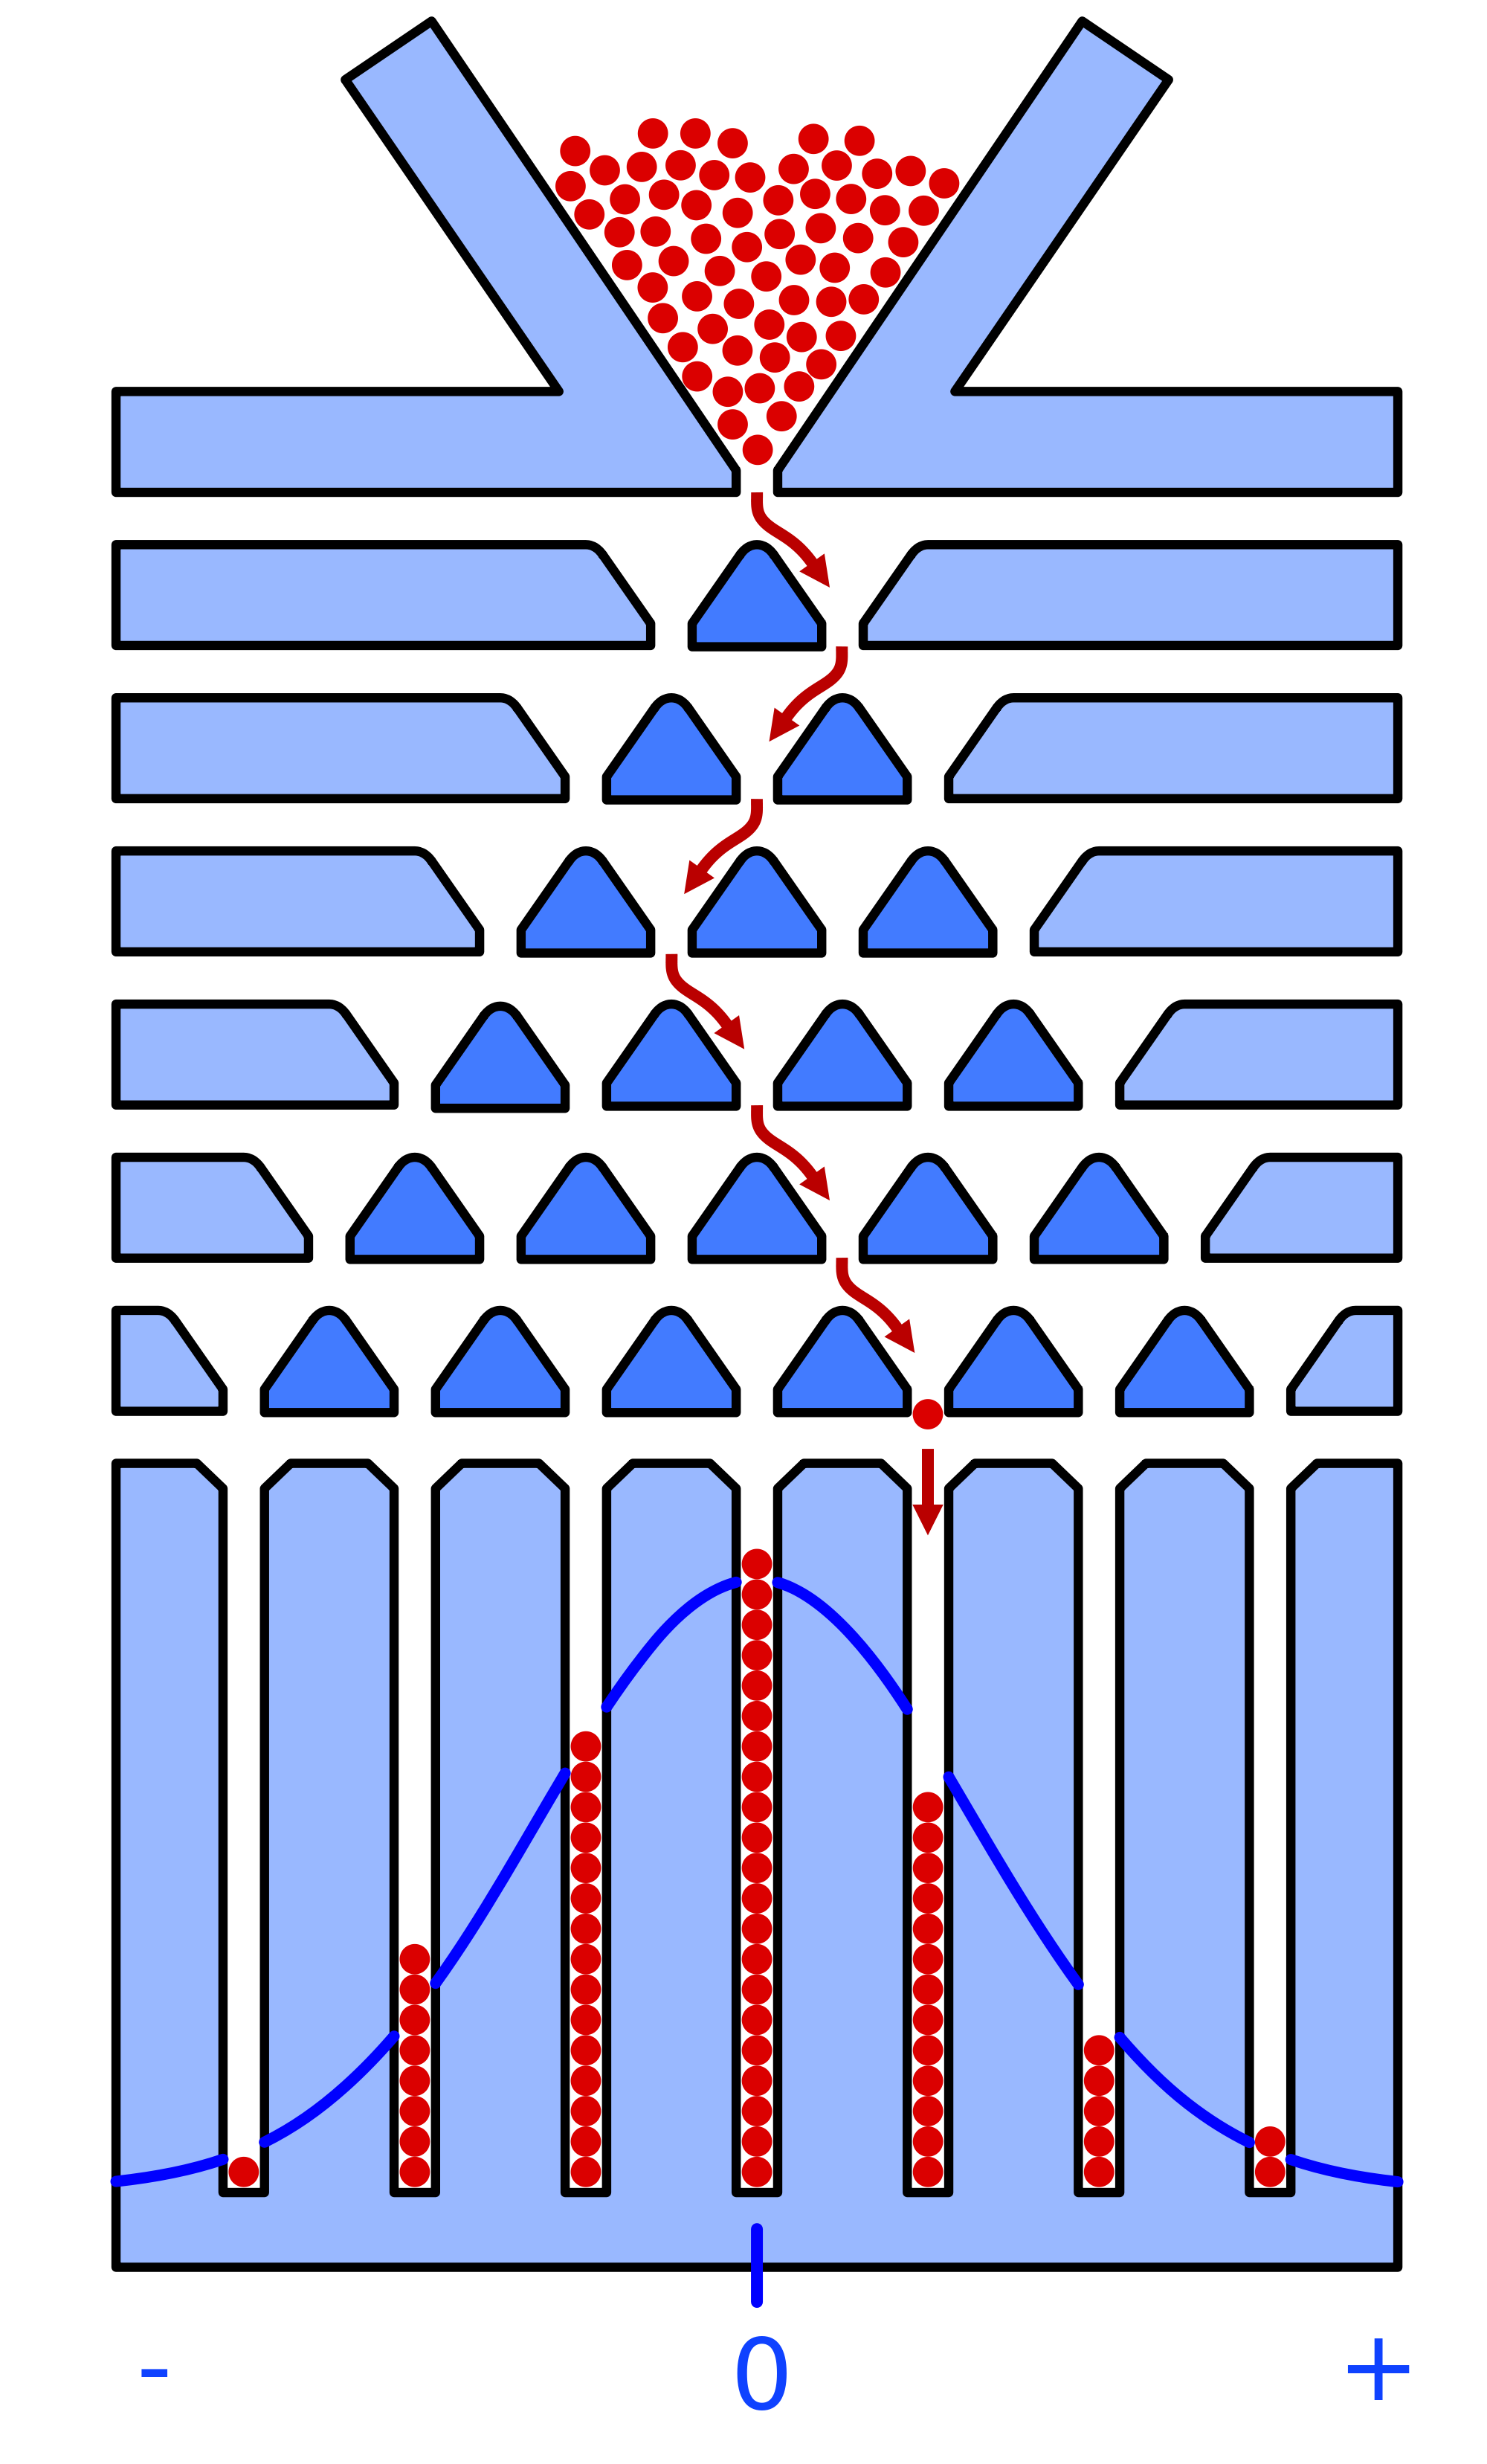
\includegraphics[scale=0.04]{img/galton.png}
\end{exercise}
\end{frame}

\begin{frame}[fragile]
\frametitle{Iteration - Exercise}
\begin{exercise}
Write a program which simulates the probability of having a blackjack (Ace and 10).
The game contains 6 sets of cards. Each set has 52 cards.\\
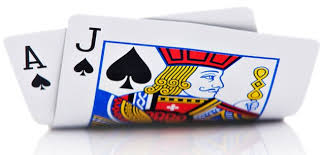
\includegraphics[scale=0.5]{img/blackjack.jpg}
\end{exercise}
\end{frame}


\begin{frame}[fragile]
  \frametitle{Jump}
  Jump statements allow altering the flow of a program by performing jumps to specific locations.
  \begin{itemize}
  \item {\bf break}\\
  break leaves a loop, even if the condition for its end is not fulfilled.
  It can be used to end an infinite loop, or to force it to end before its natural end.
  \item {\bf continue}\\
  The continue statement causes the program to skip the rest of the loop in the current iteration, as if the end of the statement block had been reached,
  causing it to jump to the start of the following iteration.
  \end{itemize}
\end{frame}

\begin{frame}[fragile]
\frametitle{Arrays}
An array is a series of elements of the same type placed in contiguous memory locations that can
be individually referenced by adding an index to a unique identifier.
\begin{lstlisting}
int a[5]; // creates 5 variables of type int
a[0] = 0;
a[1] = 1;
...
a[4] = 4;
\end{lstlisting}
ATTENTION: read or write access to an element which is not in the range of the array
end up in serious problems!
\end{frame}

\begin{frame}[fragile]
\frametitle{Arrays - Initialization}
By default, arrays are left uninitialized. This means that none of its elements are set to any particular value.
\begin{lstlisting}
int a[5] = {0, 1, 2, 3, 4};
\end{lstlisting}

Values which are not provided in the initialization list will be filled up with zeros.
\begin{lstlisting}
int b[5] = {0, 1};
\end{lstlisting}

Empty initialization list. All elements will have the value 0.
\begin{lstlisting}
int c[5] = {};
\end{lstlisting}

Array without a given size
\begin{lstlisting}
int d[] = {0, 1, 2};
\end{lstlisting}

\end{frame}

\begin{frame}[fragile]
\frametitle{Arrays - Example}
\lstinputlisting{code/array/main.cpp}
\end{frame}

\begin{frame}[fragile]
\frametitle{Arrays - Multidimension}
Arrays in C++ could have several dimensions.
\lstinputlisting{code/array/multiarray.cpp}
\end{frame}

\begin{frame}[fragile]
\frametitle{Strings}
A string is traditionally a sequence of characters. C++ provides two types for string representations:
\begin{itemize}
\item C-Style character array
\item String class from C++ Standard
\end{itemize}
\end{frame}

\begin{frame}[fragile]
\frametitle{Strings - Character Array}
The C-style character string (\verb|#include<cstring>|) originated within the C language and continues to be supported within C++.
This string is actually a one-dimensional array of characters which is terminated by a null
character \verb|\0|.
\begin{lstlisting}
char s1[6] = {'H', 'e', 'l', 'l', 'o', '\0'};
char s2[] = "Hello";
\end{lstlisting}
Several operations are available, e.g. \verb|strcpy|, \verb|strcat|, \verb|strlen|, ...
\end{frame}

\begin{frame}[fragile]
\frametitle{Strings - String class}
The standard C++ library (\verb|#include<string>|) provides a string class that supports much more operations
as the old C-String.
\begin{lstlisting}
string s1 = "Hello";
string s2 = "World";
cout << s1.size() << endl;
\end{lstlisting}
A more detailed introduction to strings will be part in the STL chapter.
\end{frame}

\begin{frame}[fragile]
\frametitle{Strings - Exercise}
\begin{exercise}
Write a program which takes a string as input. The string contains a set of pairs. Each
pair contains a number and a character: \verb|2n3m5x| (3 pairs: 2n, 3m and 5x).\\
The program should now encode this string by writing all character the given amount
of times.\\
\verb|2n3m5x| will be \verb|nnmmmxxxxx|.
\end{exercise}
\end{frame}

\begin{frame}[fragile]
\frametitle{Pointers}
When a variable is declared, the memory needed to store its value to a specific location in memory.
The exact position is defined by the operating system. However, it may be useful for a program to be
able to obtain the memory address of a variable during runtime in order to access data cells that
are at a certain position relative to it.\\
\vspace{3mm}
The address operator \verb|&| is used to find out the address in memory of a variable.

{\tiny
\begin{lstlisting}
int n = 5; // integer variable
int *p; // pointer variable. Stores the address of an integer variable
p = &n; // Stores the address of n into p
cout << p << endl; // print the address of n
\end{lstlisting}
}
\end{frame}

\begin{frame}[fragile]
\frametitle{Pointers}
The dereference operator \verb|*| is used to access a variable by using its address.

{\tiny
\begin{lstlisting}
int n = 5; // integer variable
int *p; // pointer variable. Stores the address of an integer variable
p = &n; // Stores the address of n into p
n = 20; // Stores 20 in n by using the variable name
*p = 25; // Stores 25 in n by using the variable address
\end{lstlisting}
}
\end{frame}

\begin{frame}[fragile]
\frametitle{Pointers}
Defining pointer variables:
{\tiny
\begin{lstlisting}
int *p; // defines a pointer to store the address of a int variable
int *n, m; // n is a pointer, m is NOT a pointer
float *fp; // defines a pointer to store the address of a float variable
\end{lstlisting}
}
\end{frame}

\begin{frame}[fragile]
\frametitle{Pointers}
In principle, pointers are meant to point to valid addresses,
such as the address of a variable or the address of an element in an array.
But pointers can actually point to any address,
including addresses that do not refer to any valid element. 
{\tiny
\begin{lstlisting}
int *p; // undefined pointer
*p = 5;
\end{lstlisting}
}
Accessing such a pointer causes undefined behavior,
ranging from an error during runtime to accessing some random value.
\end{frame}

\begin{frame}[fragile]
\frametitle{Pointers}
But, sometimes, a pointer really needs to explicitly point to nowhere, and not just an invalid address.
For such cases, there exists a special value that any pointer type can take:
the null pointer value.
{\tiny
\begin{lstlisting}
int *p;
p = 0;
p = nullptr;
p = NULL;
\end{lstlisting}
}
Accessing such a pointer causes undefined behavior,
ranging from an error during runtime to accessing some random value.
\end{frame}

\begin{frame}[fragile]
\frametitle{Dynamic Memory}
In the programs seen in previous slides, all memory needs were determined
before program execution by defining the variables needed.
But there may be cases where the memory needs of a program can only be determined during runtime.

\begin{lstlisting}
int *p = null; // pointer variable
p = new int;
// creates a new integer variable,
// p will now point to this variable
\end{lstlisting}

\begin{lstlisting}
int *p = null; // pointer variable
p = new int[5];
// creates a new integer array,
// p will now point to p[0]
\end{lstlisting}

\end{frame}

\begin{frame}[fragile]
\frametitle{Dynamic Memory}
Dynamic memory is in most cases only needed for a specific period of time within
the program. The allocated memory needs then to be released.

\begin{lstlisting}
int *p = null; // pointer variable
p = new int;
// some code
delete p;
// the memory to which p points will be
// released. The pointer p will still exist.
\end{lstlisting}
\end{frame}

\begin{lstlisting}
int *p = null; // pointer variable
p = new int[5];
// some code
delete [] p;
\end{lstlisting}

\begin{frame}[fragile]
\frametitle{Dynamic Memory}
Memory Leaks:

\begin{lstlisting}
int *p = null; // pointer variable
p = new int;
// some code
p = new int;
\end{lstlisting}
In the above code, the first allocated memory will be lost
after the second allocation.\\
This means that the variable is still in there, but unknown where
in the memory. This is called \bf{Memory Leak}.

\end{frame}

\begin{frame}[fragile]
\frametitle{References}
A reference variable is an alias, that is, another name for an already existing
variable.
\begin{lstlisting}
int i = 17;
int &r = i;
\end{lstlisting}
\end{frame}

\begin{frame}[fragile]
\frametitle{References}
A reference is different than a pointer:
\begin{itemize}
\item NULL references are not possible. A reference is always connected to a piece of storage.
\item Once a reference is initialized to an object, it cannot be changed to refer to another object.
\item A reference must be initialized when it is created.
\end{itemize}
\end{frame}

\begin{frame}[fragile]
\frametitle{Can you remember? Duke Nukem 3D}
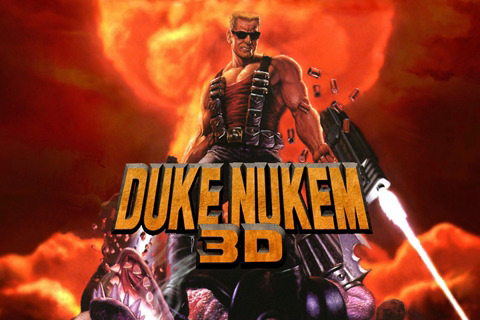
\includegraphics[scale=0.3]{img/dukenukem.jpg}
\begin{exercise}
Take a look on the source code of this game and explain a piece of code
in detail.
\end{exercise}
\end{frame}


%\section{Memory Management}
\begin{frame}[fragile]
  \frametitle{Memory Management}
\end{frame}


\subsection{Command Line Arguments}

\begin{frame}[fragile]
\frametitle{Command Line Arguments}
\begin{lstlisting}
int main(int argc, char **argv) { ... }
\end{lstlisting}
argc: Argument Count\\
argv: Argument Values / Vector
\vspace{3mm}
{\tiny
\begin{lstlisting}
int main(int argc, char **argv) {
  cout << argc << endl;
  for (int i=0; i<argc; i++) {
	cout << argv[i] << endl;
  }
  return 0;
}
\end{lstlisting}
\verb|a.out v1 v2 "v3 v4"|\\
\vspace{3mm}
a.out\\
v1\\
v2\\
v3 v4\\
}
\end{frame}

\section{OOP - Object Oriented Programming}

\begin{frame}[fragile]
\frametitle{Object Oriented Programming}
Object oriented programming is a programming paradigm based on the concept of objects,
which may contain data, known as attributes; and code, known as methods.\\
The most important features are:
\begin{itemize}
\item Classes and Objects
\item Data Encapsulation
\item Inheritance
\item Polymorphism
\end{itemize}
\end{frame}

\begin{frame}[fragile]
\frametitle{Classes}
A class contains a description (building plan). This building plan describes how
objects of this class will be created.
{\tiny
\begin{lstlisting}
class Fraction {
public:
  int numerator;
  int denominator;
};
	
int main() {
  Fraction f1, f2; // f1 & f2 are objects
  f1.numerator = 1; // set numerator
  f1.denominator = 2; // set denominator
  f2.numerator = 3;
  f2.denominator = 4;
  return 0;
}
\end{lstlisting}
}
\end{frame}

\begin{frame}[fragile]
\frametitle{Methods}
\end{frame}

\begin{frame}[fragile]
\frametitle{Method Overloading}
\end{frame}

\begin{frame}[fragile]
\frametitle{Constructor}
\end{frame}

\begin{frame}[fragile]
\frametitle{Copyconstructor}
\end{frame}

\begin{frame}[fragile]
\frametitle{Destructor}
\end{frame}

\begin{frame}[fragile]
\frametitle{Public, Private}
\end{frame}

\begin{frame}[fragile]
\frametitle{Data Encapsulation}
\end{frame}

\begin{frame}[fragile]
\frametitle{Static}
\end{frame}

\begin{frame}[fragile]
\frametitle{Static Questions}
\begin{exercise}
\begin{enumerate}
\item Is a static member accessible by a non static method?
\item Is a non static member accessible by a static method?
\end{enumerate}
\end{exercise}
\end{frame}


\subsection{Inheritance}

\begin{frame}[fragile]
\frametitle{Inheritance}
{\small
Classes in C++ can be extended, creating new classes which retain characteristics of the base class.
This process, known as inheritance, involves a base class and a derived class: The derived class
inherits the members of the base class, on top of which it can add its own members.
\begin{lstlisting}
class A { // Base class
};

class B : public A { // Derived class
};
\end{lstlisting}
}
\end{frame}

\begin{frame}[fragile]
\frametitle{Inheritance - Constructor}
{\tiny
\lstinputlisting{code/inheritance/constructor.cpp}
Output:\\
\verb|Constructor A|\\
\verb|Constructor B|\\
The base constructor will be executed {\bf\emph{before}} the constructor of the derived class.
}
\end{frame}

\begin{frame}[fragile]
\frametitle{Inheritance - Constructor}
If nothing specific is defined, the contructor with no arguments will be taken
from the super class.
{\tiny
\lstinputlisting{code/inheritance/constructor2.cpp}
Output:\\
\verb|Constructor A|\\
\verb|Constructor B with arg|\\
}
\end{frame}

\begin{frame}[fragile]
\frametitle{Inheritance - Constructor}
A compiler error will occure, if a constructor with no arguments
is not available.
{\tiny
\lstinputlisting{code/inheritance/constructor3.cpp}
\bf{Compiler Error}
}
\end{frame}

\begin{frame}[fragile]
\frametitle{Inheritance - Constructor}
The constructor of the sub class needs to define which constructor of the
super class should be used.
{\tiny
\lstinputlisting{code/inheritance/constructor4.cpp}
Output:\\
\verb|Constructor A with arg|\\
\verb|Constructor B with arg|\\
}
\end{frame}

\begin{frame}[fragile]
\frametitle{Inheritance - Destructor}
{\tiny
\lstinputlisting{code/inheritance/destructor.cpp}
Output:\\
\verb|Destructor B|\\
\verb|Destructor A|\\
The base destructor will be executed {\bf\emph{after}} the destructor of the derived class.
}
\end{frame}

\begin{frame}[fragile]
\frametitle{Inheritance - Protected}
\end{frame}

\begin{frame}[fragile]
\frametitle{Inheritance - Polymorphism}
{\tiny
One of the key features of class inheritance is that a pointer to a derived class is type-compatible
with a pointer to its base class. Polymorphism is the art of taking advantage of this simple but
powerful feature.
\lstinputlisting{code/inheritance/polymorphism1.cpp}
Output:\\
\verb|Method class A|\\
This output is NOT CORRECT!. As the pointer points to an object of class B,
the method of class B should be executed!. To avoid this failure, the method
in the base class must be declared as \verb|virtual|.
}
\end{frame}

\begin{frame}[fragile]
\frametitle{Inheritance - Polymorphism}
{\tiny
\lstinputlisting{code/inheritance/polymorphism2.cpp}
Output:\\
\verb|Method class B|\\
This output is CORRECT!. A method declared as \verb|virtual| will be checked at runtime,
to find out the correct class on which the method should be executed.
Therefore a non-virtual declared method should not be overwritten.
}
\end{frame}

\begin{frame}[fragile]
\frametitle{Inheritance - Polymorphism}
{\tiny
\lstinputlisting{code/inheritance/polymorphism3.cpp}
Output:\\
\verb|Destructor class A|\\
This output is NOT CORRECT!. As the object is from class B, the destructor
of class B should also be called. To avoid this failure, the destructor in
the base class must be declared as \verb|virtual|. 
}
\end{frame}

\begin{frame}[fragile]
\frametitle{Inheritance - Polymorphism}
{\tiny
\lstinputlisting{code/inheritance/polymorphism4.cpp}
Output:\\
\verb|Destructor class B|\\
\verb|Destructor class A|\\
This output is CORRECT!. Therefore a class should never be inherited if there is
a non-virtual destructor.
}
\end{frame}

\begin{frame}[fragile]
\frametitle{Inheritance - Abstract class}
{\tiny
Abstract base classes can only be used as base classes, and thus are allowed to have virtual member functions
without definition (known as pure virtual functions).
\lstinputlisting{code/inheritance/abstract.cpp}
It is not possible to create an object of an abstract base class. If a derived class does not
override all pure virtual methods, the derived class is also abstract (without pure virtual
methods).
}
\end{frame}

\subsection{Rule of Three}

\begin{frame}[fragile]
	\frametitle{Rule of three}
	The rule of three is a rule of thumb in C++ that claims that if a class defines one of the following
	it should probably explicitly define all three!
	\begin{itemize}
	\item Destructor
	\item Copy constructor
	\item Assignment operator
	\end{itemize}
\end{frame}

\begin{frame}[fragile]
	\frametitle{Rule of three}
	{\tiny
	\lstinputlisting{code/ruleofthree/source.h}
	}
\end{frame}

\begin{frame}[fragile]
	\frametitle{Rule of three}
	{\tiny
	\lstinputlisting{code/ruleofthree/source.cpp}
	}
\end{frame}
\subsection{Templates}
\begin{frame}[fragile]
\frametitle{Templates}
Templates are a feature of the C++ language that allows functions and classes to operate
with generic types. This allows a function of class to work on many different data types
without being rewritten for each one.
{\tiny
\begin{lstlisting}
int minimum(int a, int b) {
  if (a < b) return a;
  return b;
}

double minimum(double x, double y) {
  if (x < y) return x;
  return y;
}

A minimum(A obj1, A obj2) {
  // ATTENTION: class A must overload < operator!
  if (obj1 < obj2) return obj1;
  return obj2;
}
\end{lstlisting}
}
The function \verb|minimum| must only be written once if templates are used.
\end{frame}

\begin{frame}[fragile] 
\frametitle{Function templates}
{\tiny
\begin{lstlisting}
template <class T>
T minimum(T a, T b) {
  if (a < b) return a;
  return b;
}

int main(int argc, char **argv) {
  // use function for type integer
  int a=5, b=6;
  int c = minimum<int>(a, b);

  // use function for type double
  double x=3.1, y=5.4;
  double z = minimum<double>(a, b);
  
  // use function for type string
  string s1 = "Hello";
  string s2 = "World";
  string s = minimum<string>(s1, s2);

  return 0;
}
\end{lstlisting}
}
\end{frame}

\begin{frame}[fragile] 
\frametitle{Function templates}
{\tiny
\begin{lstlisting}
template <class T>
T minimum(T a, T b) {
  if (a < b) return a;
  return b;
}

class A {
  // some implementation
};

int main(int argc, char **argv) {
  // use function for type A
  A obj1, obj2;
  A result = minimum<A>(obj1, obj2);
  
  return 0;
}
\end{lstlisting}
}
This will end up in a compiler error, because class A does
not overload the \verb|operator <|!
\end{frame}

\begin{frame}[fragile] 
\frametitle{Function templates}
{\tiny
\begin{lstlisting}
template <class T>
T min(T a, T b) {
  if (a < b) return a;
  return b;
}

class A {
  // some implementation
public:
  bool operator< (const A & obj);
};

int main(int argc, char **argv) {
  // use function for type A
  A obj1, obj2;
  A result = min<A>(obj1, obj2);
  
  return 0;
}
\end{lstlisting}
}
\end{frame}

\begin{frame}[fragile] 
\frametitle{Class templates}
{\tiny
\begin{lstlisting}
template <class T>
class Container {
private:
  T value;
public:
  T getValue();
  void setValue(T value);
};

template <class T>
T Container<T>::getValue() {
  return value;
}

template <class T>
void Container<T>::setValue(T value) {
  this->value = value;
}

int main(int argc, char **argv) {
  // use class for type double
  Container<double> obj;
  double x = 3.1;
  obj.setValue(x);
  
  return 0;
}
\end{lstlisting}
}

\end{frame}


\section{STL - Standard Template Library}

\begin{frame}[fragile]
  \frametitle{STL - Standard Template Library}
  \begin{itemize}
  \item Containers\\
  {\small STL contains sequence containers, associative containers and container adaptors}
  \item Iterators\\
  {\small STL contains input iterators, output iterators, forward iterators, bidirectional iterators and random access iterators}
  \item Algorithms\\
  {\small STL contains a large number of algorithms (e.g. sorting, searching)}
  \end{itemize}
\end{frame}

\begin{frame}[fragile]
  \frametitle{STL - Containers}
  Sequence Container
  {\small
  \begin{itemize}
  \item vector
  \item deque
  \item list
  \item array (C++11)
  \end{itemize}
  Adaptive Containers
  \begin{itemize}
  \item stack
  \item queue
  \end{itemize}
  Associative Containers (elements are in order)
  \begin{itemize}
  \item map, multimap
  \item set, multiset
  \end{itemize}
  \verb|http://www.cplusplus.com/reference/|
  }
\end{frame}

\begin{frame}[fragile]
\frametitle{Vector, Deque, List}
{\tiny
\begin{lstlisting}
int main(int argc, char **argv) {

  deque<int> c1;
  vector<int> c2;
  list<int> c3;

  // insert at the end
  c1.push_back(rand());
  c2.push_back(rand());
  c3.push_back(rand());

  // insert at the start
  c1.push_front(rand());
  // c2.push_front not possible
  c3.push_front(rand());
\end{lstlisting}
}
\end{frame}

\begin{frame}[fragile]
\frametitle{Vector, Deque, List}
{\tiny
\begin{lstlisting}
  // insert at a specific position
  list<int>::iterator iter3 = c3.begin();
  iter3++;
  c3.insert(iter3, rand());

  // delete at a specific position
  vector<int>::iterator iter2 = c2.begin();
  c2.erase(iter2);

  // loop through elements
  deque<int>::iterator iter1;
  for (iter1=c1.begin(); iter1!=c1.end(); iter1++) {
    cout << *iter1 << endl;
  }

  return 0;
}
\end{lstlisting}
}
\end{frame}

\begin{frame}[fragile]
  \frametitle{Performance Comparison}
  {\tiny
  Deque
  \begin{verbatim}
Time (push_back, 10 Mio Elements): 0.123527
Time (insert, 1000 Elements): 11.0062
Time (erase, 1000 Elements): 10.9873
  \end{verbatim}
  Vector
  \begin{verbatim}
Time (push_back, 10 Mio Elements): 0.166174
Time (insert, 1000 Elements): 2.12804
Time (erase, 1000 Elements): 2.09296
  \end{verbatim}
  List
  \begin{verbatim}
Time (push_back, 10 Mio Elements): 0.806527
Time (insert, 1000 Elements): 8.5e-05
Time (erase, 1000 Elements): 6.7e-05
  \end{verbatim}
  }
\end{frame}

\begin{frame}[fragile]
\frametitle{Map}
{\tiny
\begin{lstlisting}
map<int, string> employeeMap;

// insert
employeeMap[0] = "HERZIG";
employeeMap[1] = "BALE";
employeeMap[0] = "WAYNE"; // old value will be overwritten

pair<map<int, string>::iterator, bool> ret;
ret = employeeMap.insert(pair<int, string>(2, "PARKER"));
// ret.second is true
ret = employeeMap.insert(pair<int, string>(2, "CLARK"));
// ret.second is false, because key 2 already exists

// loop through elements
map<int, string>::iterator iter;
for (iter=employeeMap.begin(); iter!=employeeMap.end(); iter++) {
  int key = iter->first;
  string value = iter->second;
}
\end{lstlisting}
}
\end{frame}

\begin{frame}[fragile]
\frametitle{Set}
{\tiny
\begin{lstlisting}
set<int> data;

pair<set<int>::iterator,bool> ret;
for (int i=0; i<100; i++) {
  int number = rand() % 100;
  ret = data.insert(number);
  if (!(ret.second)) {
    cout << "Could not insert " << number << endl;
  }
}
cout << data.size() << endl;

set<int>::iterator it;
for (it=data.begin(); it!=data.end(); it++) {
  cout << *it << endl;
}
\end{lstlisting}
}
\end{frame}

\begin{frame}[fragile]
\frametitle{STL - Algorihtms}
The algorithms library defines functions for a variety of purposes (e.g. searching, sorting,
counting, manipulating) that operate on ranges of elements. Note that a range is defined as
\verb|[first, last)| where last refers to the element past the last element to inspect or modify.
\begin{itemize}
\item Non-modifying sequence operations
\item Modifying sequence operations
\end{itemize}

\end{frame}

\begin{frame}[fragile]
\frametitle{count}
{\tiny
Sucht nach einem bestimmten Element in einem
Container und gibt die Anzahl der Vorkommnisse zurück.

\lstinputlisting{code/stl/count.cpp}

\emph{Ähnliche Algorithmen}: \verb|count_if|
}
\end{frame}

\begin{frame}[fragile]
\frametitle{all\_of}
{\tiny
Prüft ob eine Bedinung für alle Elemente wahr ist.\\
\emph{ACHTUNG:} Teil von \verb|C++0x|, (\verb|g++ -std=c++0x file.cpp|).

\lstinputlisting{code/stl/allof.cpp}

\emph{Ähnliche Algorithmen}: \verb|any_of, none_of|
}
\end{frame}

\begin{frame}[fragile]
\frametitle{find}
{\tiny
Sucht nach einem Element im Container und gibt den Iterator auf dieses Element zurück.
Kommt das Element im Container nicht vor, so ist der Rückgabewert gleich \verb|container.end()|.

\lstinputlisting{code/stl/find.cpp}

\emph{Ähnliche Algorithmen}: \verb|find_if, find_if_not, find_end, find_first_of|
}
\end{frame}

\begin{frame}[fragile]
\frametitle{is\_permutation}
{\tiny
Prüft zwei Container ob die gleichen Elemente vorkommen. Egal in welcher Reihenfolge.\\
\emph{ACHTUNG:} Teil von \verb|C++0x|, (\verb|g++ -std=c++0x file.cpp|).

\lstinputlisting{code/stl/permutation.cpp}
}
\end{frame}

\begin{frame}[fragile]
\frametitle{copy}
{\tiny
Kopiert die Elemente aus einem Container in einen anderen. Der Ziel Container muss
dafür entsprechend Platz zur Verfügung stellen.

\lstinputlisting{code/stl/copy.cpp}
}
\end{frame}

\begin{frame}[fragile]
\frametitle{move}
{\tiny
\emph{ACHTUNG:} Teil von \verb|C++0x|, (\verb|g++ -std=c++0x file.cpp|).

\lstinputlisting{code/stl/move.cpp}
}
\end{frame}

\begin{frame}[fragile]
\frametitle{replace}
{\tiny
Ein Element durch ein anderes Element ersetzen.

\lstinputlisting{code/stl/replace.cpp}
}
\end{frame}

\begin{frame}[fragile]
\frametitle{fill}
{\tiny
Fügt allen Elementen eines Containers einen bestimmten Wert zu.

\lstinputlisting{code/stl/fill.cpp}
}
\end{frame}

\begin{frame}[fragile]
\frametitle{unique}
{\tiny
Entfernt alle aufeinanderfolgenden Duplikate (ausser das erst gefundene) aus einem Container.
Die Grösse muss nach dem Entfernen manuell angepasst werden. Dazu kann der Rückgabewert
verwendet werden. Dies ist ein Iterator auf das letzte gültige Element.

\lstinputlisting{code/stl/unique.cpp}
}
\end{frame}

\begin{frame}[fragile]
\frametitle{shuffle}
{\tiny
Durchmischt die Elemente eines Containers.
\emph{ACHTUNG:} Teil von \verb|C++0x|, (\verb|g++ -std=c++0x file.cpp|).

\lstinputlisting{code/stl/shuffle.cpp}
}
\end{frame}

\begin{frame}[fragile]
\frametitle{min\_element}
{\tiny
Sucht nach dem Minimum in einem Container.

\lstinputlisting{code/stl/minelement.cpp}
}
\end{frame}

\begin{frame}[fragile]
\frametitle{min, max}
{\tiny
Template Funktion um den kleineren resp. grösseren Wert zweier Parameter
zu bestimmen.

\lstinputlisting{code/stl/min.cpp}
}
\end{frame}

\begin{frame}[fragile]
\frametitle{sort}
{\tiny
Sortiert alle Elemente in einem Container.

\lstinputlisting{code/stl/sort.cpp}
}
\end{frame}

\begin{frame}[fragile]
\frametitle{Exercise}
{\tiny
\begin{exercise}
Insert 10000 random numbers (0..10000) into a vector. Write a program which counts
the number of different numbers (e.g. 1, 2, 1, 3, 2: contains 3 elements)
\end{exercise}
\begin{exercise}
Insert 10000 random numbers (0..10000) into a vector. Remove all even numbers.
\end{exercise}
\begin{exercise}
Insert 100 numbers (in order: 0,1,2,...) into a vector. Shuffle that vector.
\end{exercise}
\begin{exercise}
Insert 500 random numbers (0..1000) into a vector v1 and into a vector v2. Print
out all numbers which are only in v1 and v2.
\end{exercise}
}
\end{frame}

\section{Algorithms and Datastructures}
\begin{frame}[fragile]
\frametitle{Algorihtms and Datastructures}
\begin{displaymath}
Computer Program = Algorithms + Data Structures
\end{displaymath}
\begin{itemize}
\item Introduction
\item Analysis
\item Algorithmic Toolbox
\item Basic Data Structures
\item Sorting and Searching
\item Trees and Tree Algorithms
\item Graphs and Graph Algorithms
\item String Algorithms
\end{itemize}
\end{frame}

\subsection{Time Measurement}
\begin{frame}[fragile]
\frametitle{Time Measurement}
C++ provides possibilities to measure the time consumption of a given
code fragment. To use these possibilities, the header file \verb|ctime|
must be included.

{\tiny
\begin{lstlisting}
#include <ctime>
#include <iostream>
using namespace std;

int main(int argc, char **argv) {
  clock_t start, stop;
  start = clock();

  // CODE FRAGMENT

  stop = clock();
  // Time in seconds
  double time = (double)(stop-start)/CLOCKS_PER_SEC;
}
\end{lstlisting}
}
\end{frame}

\begin{frame}[fragile]
\frametitle{Time Measurement - Exercise}
{\tiny
\begin{exercise}
Measure the time needed for the following code fragment on your computer.
\begin{lstlisting}
int main(int argc, char **argv) {
  string s = // some random string containing [A-Z]
  int result[26];
  for (int i=0; i<26; i++) {
    int counter = 0;
    char ch = 'A' + i;
    for (int j=0; j<s.size(); j++) {
      if (s.at(j) == ch) counter++;
    }
    result[i] = counter;
  }
  for (int i=0; i<26; i++) {
    cout << ((char)('A'+i)) << " : " << result[i] << endl;
  }
  return 0;
}
\end{lstlisting}
\end{exercise}
\begin{exercise}
Find out the specification of your computer: \emph{Operating System, CPU, RAM}.
\end{exercise}
\begin{exercise}
What are the possibilities to improve the execution time?
\end{exercise}
\begin{exercise}
What are the possibilities to improve the execution time (without changing the code)?
\end{exercise}
}
\end{frame}

\begin{frame}[fragile]
\frametitle{Time Measurement}
Results:\\
\vspace{3mm}
\begin{tabular}{c|c|c|c|c}
Name & Time & CPU & OS & RAM\\
\hline
Merz & 15.4s & i7 DualCore 3.4GHz & OSX & 16GB\\
Huber & 31s & i7 QuadCore 2.5GHz & Win8 & 6GB\\
Ammann & 11.8s & i7 OctaCore & Win10 & 32GB\\
Sommer & 15.6s & i7 QuadCore 2.5GHz & OSX & 16GB\\
Born & 24s & i7 2.5GHz & Win7 & 4GB\\
Hess & 91s & i5 Dual Core 2.5GHz &  Win8 & 8GB\\
Camenzind & 19s & i5 3.1GHz & Win10 & 8GB
\end{tabular}
\end{frame}

\begin{frame}[fragile]
\frametitle{Runtime Analysis}
Big O notation is the language for articulating how long an algorithm takes to run.
With big O notation we express the runtime in terms of how quickly it grows relative to the input.

\begin{itemize}
\item $O(1)$ - Constant
\item $O(log \, n)$ - Logaritmic
\item $O(n)$ - Linear
\item $O(n \cdot log \, n)$ - Loglinear
\item $O(n^2)$ - Quadratic
\item $O(c^n), c > 1$ - Expotential
\end{itemize}

\end{frame}

\begin{frame}[fragile]
\frametitle{Runtime Analysis}
Small input size\\
\centering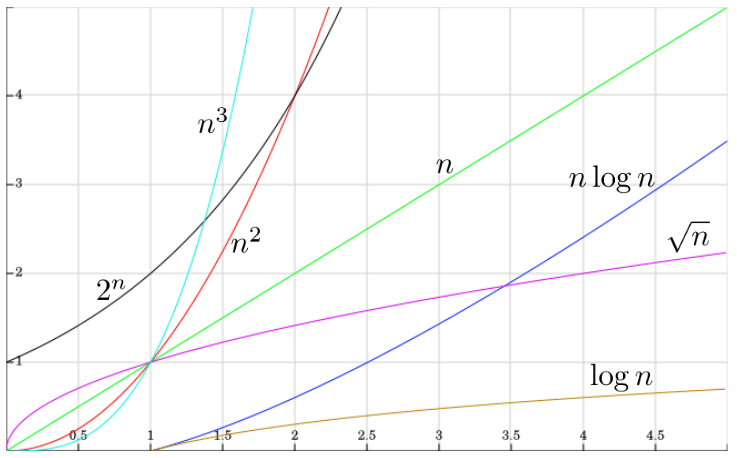
\includegraphics[scale=0.4]{img/runtime1.png}
\end{frame}

\begin{frame}[fragile]
\frametitle{Runtime Analysis}
Large input size\\
\centering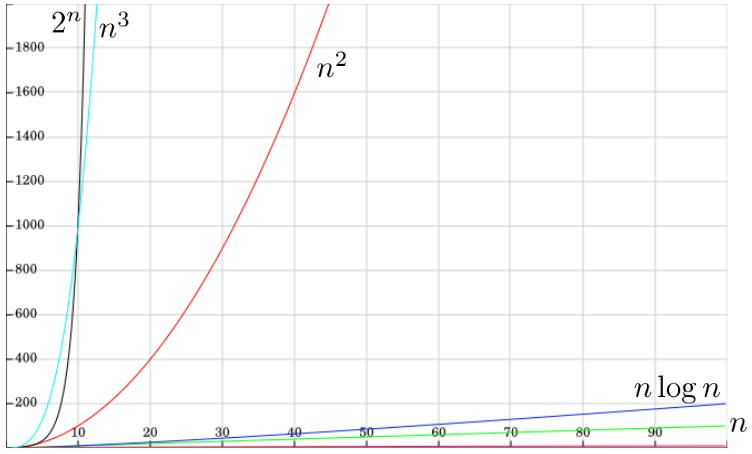
\includegraphics[scale=0.4]{img/runtime2.png}
\end{frame}

\begin{frame}[fragile]
\frametitle{Runtime Analysis}
\begin{example}
The following code computes the product of a and b. What is the runtime?
\begin{lstlisting}
int product(int a, int b) {
  int sum = 0;
  for (int i=0; i<b; i++) {
    sum += a;
  }
  return sum;
}
\end{lstlisting}
\end{example}

\end{frame}

\begin{frame}[fragile]
\frametitle{Runtime Analysis}
\begin{example}
What is the runtime of \verb|method(n)|?
\begin{lstlisting}
void method(int n) {
  for (int i=0; i<n; i++) {
    for (int j=0; j<n; j++) {
      f();
    }
}
\end{lstlisting}
\end{example}

\end{frame}

\begin{frame}[fragile]
\frametitle{DNA Analysis}
{\tiny
\begin{exercise}
Write an algorithm to find out which nucleotide appears most in the DNA
sequence of the human (chromosome 1).\\
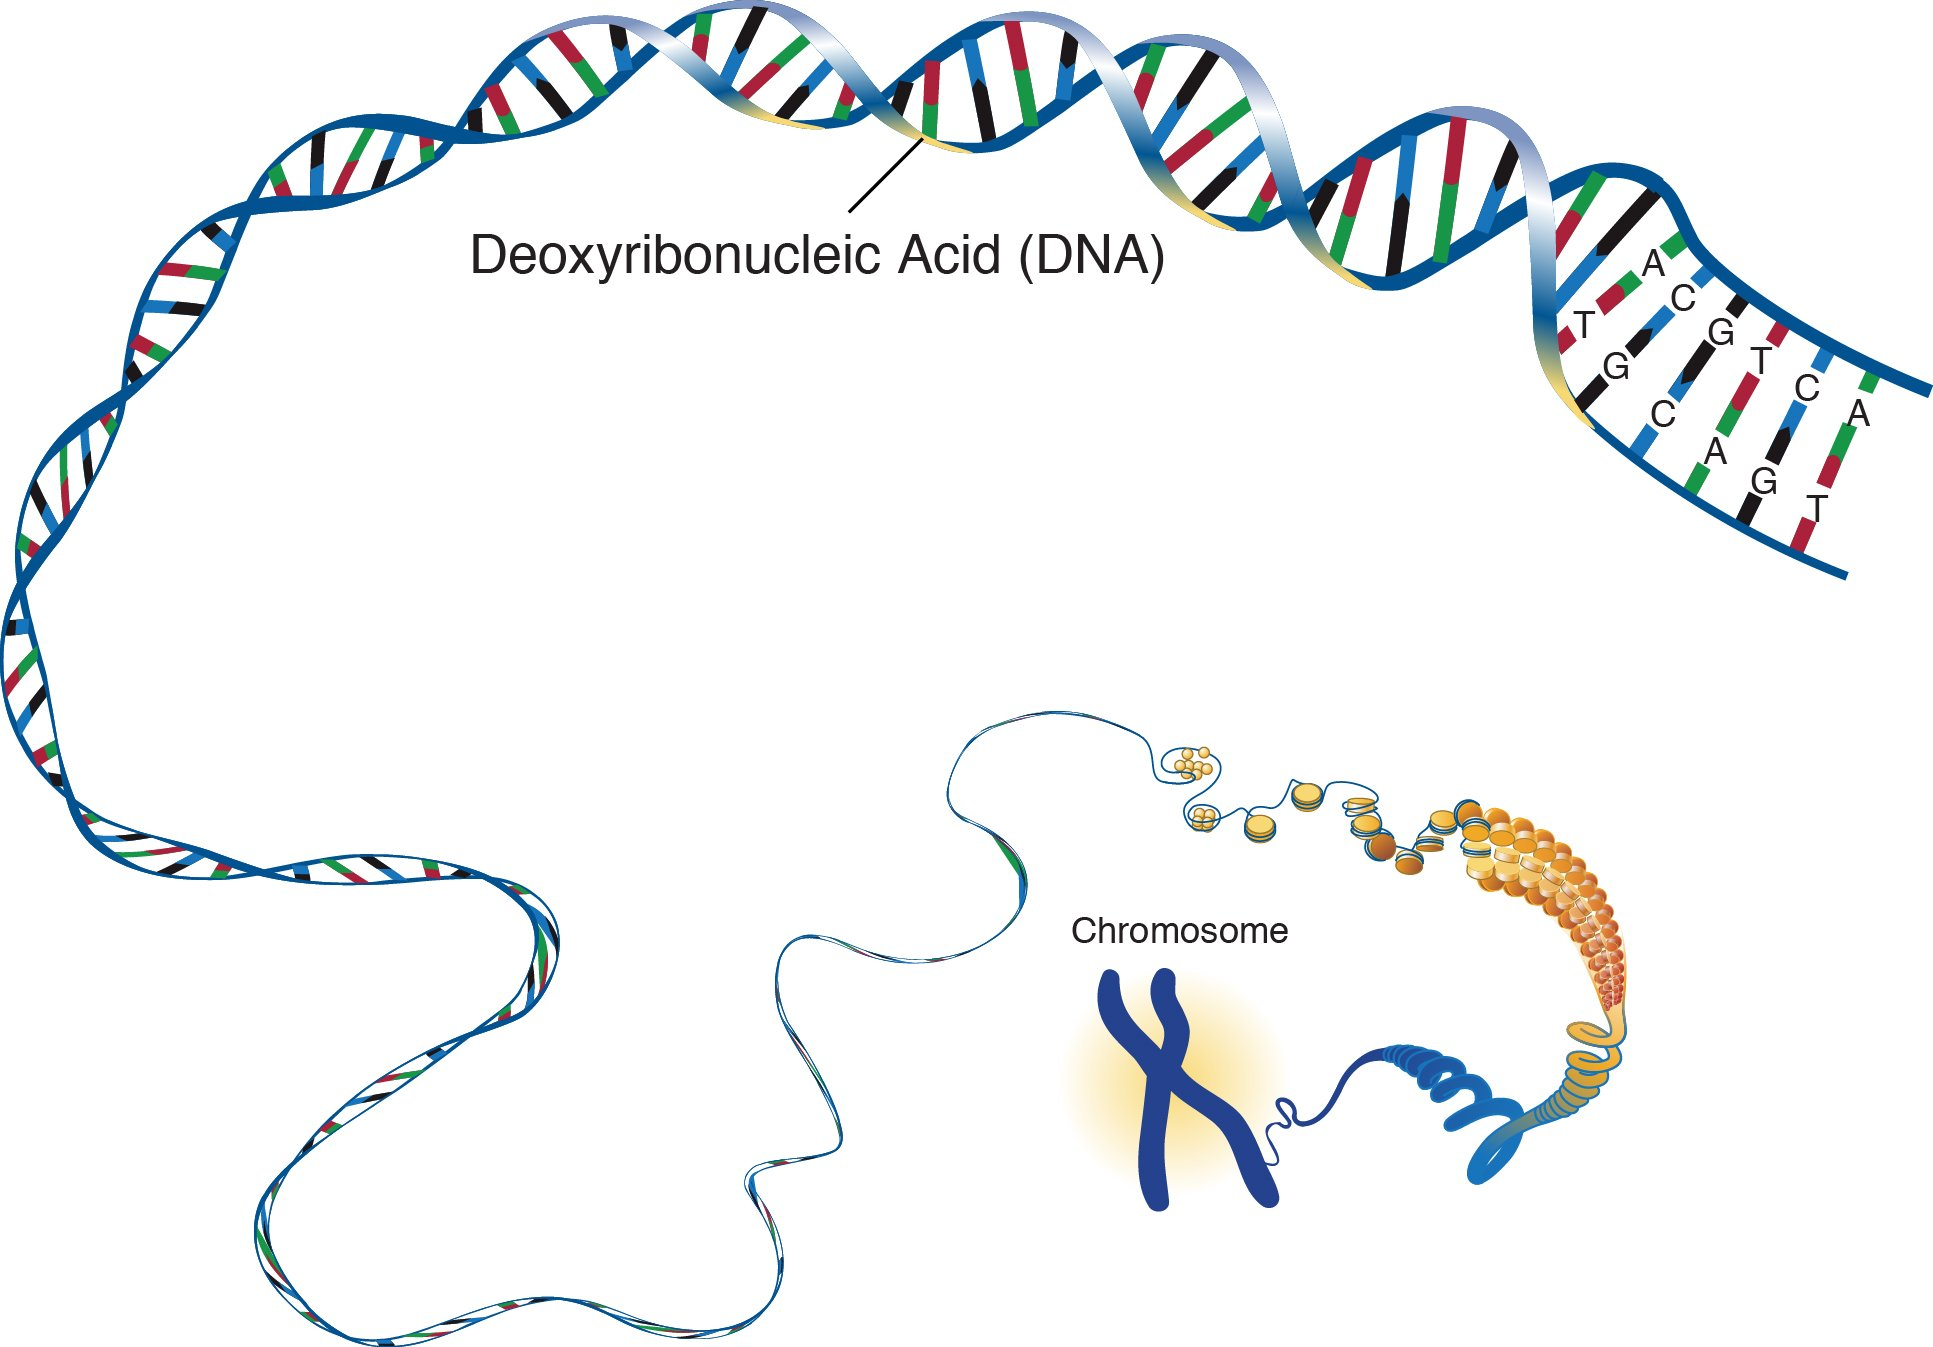
\includegraphics[scale=0.3]{img/dna.jpg}
\begin{enumerate}
\item Download the template \verb|sequence.cpp|, located on the HF-ICT share
\item Compile the code on your computer
\item Download the Human DNA Chromosome 1 sequence (fasta format) from
\verb|ftp://ftp.ncbi.nlm.nih.gov/genomes/|
\item Use the class FastaReader to read the sequence file
\item Find out the length of the sequence
\item Implement the method \verb|analyzeSequence| to find out which nucleotide
appears most.
\item Your algorihtm must run in less than 10s.
\end{enumerate}

\end{exercise}
}

\end{frame}

\begin{frame}[fragile]
\frametitle{Random Data}
\begin{exercise}
Write a class \verb|RandomDataUtil| with two methods
\begin{enumerate}
\item \verb|string createString(int size)| which creates a string, containing
random letters A-Z.
\item \verb|string createGenome(int size)| which creates a string, containing
random letters A, G, C and T.
\end{enumerate}
What is the runtime of your solution?
\end{exercise}

\end{frame}

\begin{frame}[fragile]
\frametitle{Character Frequency}
\begin{exercise}
Write a method, which takes a string (contains A-Z) as parameter. This method
should return the first character, which appears only one time
in this string.\\
What is the runtime of your solution?
\end{exercise}

\end{frame}

%\subsection{Recursion}

\begin{frame}[fragile]
\frametitle{Recursion}
\begin{figure}[h]
\centering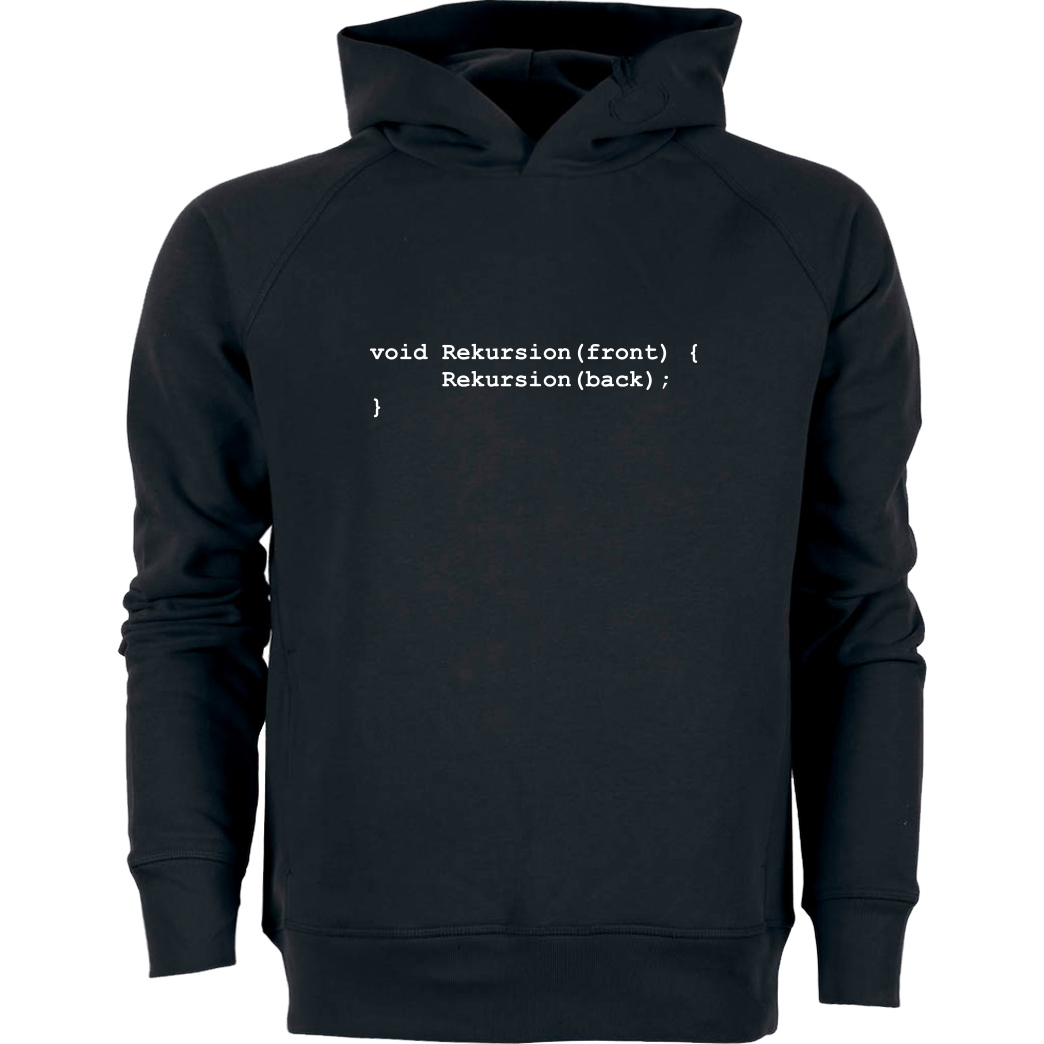
\includegraphics[scale=0.15]{img/recursion.jpg}
\caption{Recursion}
\end{figure}
\end{frame}

\begin{frame}[fragile]
\frametitle{Factorial}

\begin{definition}[Factorial]
\begin{align}
n! = 1 \cdot 2 \cdot ... \cdot (n-1) \cdot n
\end{align}
\end{definition}

\begin{definition}[Factorial Recursive]
\begin{align}
n!=\left\{\begin{aligned} & 1 & & n=0\\
& n \cdot (n-1)! & & n>0 \end{aligned}\right.
\end{align}
\end{definition}
\end{frame}

\begin{frame}[fragile]
\frametitle{Factorial}
{\tiny
\lstinputlisting{code/rekursion/fakultaet.cpp}
}
Runtime: $O(n)$
\end{frame}

\begin{frame}[fragile]
\frametitle{Factorial - Exercise}
\begin{exercise}
What is the biggest number for which the factorial could be calculated (under usage
of the code above)?
\end{exercise}
\end{frame}

\begin{frame}[fragile]
\frametitle{Fibonacci Numbers}
\begin{definition}[Fibonacci Zahlen]
\begin{align}
F_n=\left\{
\begin{aligned} & 0 & & n=0\\
& 1 & & n=1\\
& F_{n-1} + F_{n-2} & & n>1
\end{aligned}\right.
\end{align}
\end{definition}
\end{frame}

\begin{frame}[fragile]
\frametitle{Fibonacci Numbers}
{\tiny
\lstinputlisting{code/rekursion/fibonacci.cpp}
}
\end{frame}

\begin{frame}[fragile]
\frametitle{Fibonacci Numbers - Exercise}
\begin{exercise}
Rewrite the recursive function for calculating the fibonacci numbers to an iterative
version. Which one is faster, recursive or iterative?
\end{exercise}
\end{frame}

\begin{frame}[fragile]
\frametitle{Power}

\begin{definition}[Power]
\begin{align}
a^n = \underbrace{a \cdot a \cdot a \cdot ... \cdot a}_\text{n factors}
\end{align}
\end{definition}

\begin{definition}[Power Recursive]
\begin{align}
a^n=\left\{\begin{aligned} & a^{\frac{n}{2}} \cdot a^{\frac{n}{2}} & & \text{n even}\\
& a^{\frac{n-1}{2}} \cdot a^{\frac{n-1}{2}} \cdot a & & \text{n odd} \end{aligned}\right.
\end{align}
\end{definition}

\end{frame}

\begin{frame}[fragile]
\frametitle{Power - Iterative}
{\tiny
\lstinputlisting{code/rekursion/potenzIt.cpp}
}
Runtime: $O(n)$
\end{frame}

\begin{frame}[fragile]
\frametitle{Power - Recursive}
{\tiny
\lstinputlisting{code/rekursion/potenzRe.cpp}
}
Runtime: $O(log \, n)$
\end{frame}

\begin{frame}[fragile]
\frametitle{8 Queens Problems}
The eight queens puzzle is the problem of placing eight chess queens
on an 8x8 chessboard so that no two queens threaten each other.
\begin{figure}[h]
\centering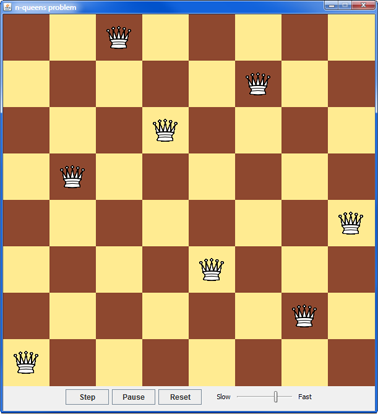
\includegraphics[scale=0.3]{img/8queens.png}
\caption{8 Queens Problems}
\end{figure}
\end{frame}

\begin{frame}[fragile]
\frametitle{8 Queens Problems}
{\tiny
\lstinputlisting{code/8queens/queenproblem.h}
}
\end{frame}

\begin{frame}[fragile]
\frametitle{8 Queens Problems}
{\tiny
\lstinputlisting{code/8queens/queenproblem.cpp}
}
\end{frame}

\begin{frame}[fragile]
\frametitle{8 Queens Problems}
{\tiny
\lstinputlisting{code/8queens/chessboard.h}
}
\end{frame}

\begin{frame}[fragile]
\frametitle{8 Queens Problems}
{\tiny
\lstinputlisting{code/8queens/main.cpp}
}
\end{frame}



%\subsection{Sorting}

\begin{frame}[fragile]
\frametitle{Sorting}

\begin{figure}[h]
\centering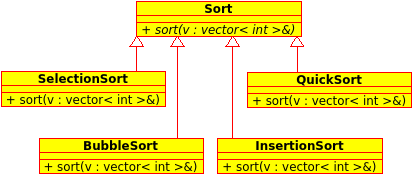
\includegraphics[scale=0.7]{img/sorting.png}
\caption{Sorting Framework}
\end{figure}

\subsubsection{Abstract class Sort}
The implementation of different sorting algorithms should be based on
the abstract Sort class as given in the following diagram:

\end{frame}

\begin{frame}[fragile]
\frametitle{Sorting}
{\small
\lstinputlisting{code/sort/sort.h}
}

\end{frame}

\begin{frame}[fragile]
\frametitle{Bubble Sort}
{\tiny
Bubble sort is a simple sorting algorithm that repeatedly steps through the list to be sorted,
compares each pair of adjacent items and swaps them if they are in the wrong order.
The pass through the list is repeated until no swaps are needed, which indicates that the
list is sorted. 
\verbatiminput{bubblesort.txt}
Runtime: $O(n^2)$
}
\end{frame}

\begin{frame}[fragile]
\frametitle{Selection Sort}
{\tiny
Selection sort divides the input list into two parts: the sublist of items already sorted,
which is built up from left to right at the front (left) of the list, and the sublist of items
remaining to be sorted that occupy the rest of the list. Initially, the sorted sublist is empty and the
unsorted sublist is the entire input list. The algorithm proceeds by finding the smallest element in the
unsorted sublist, exchanging (swapping) it with the leftmost unsorted element (putting it in sorted order),
and moving the sublist boundaries one element to the right.
\verbatiminput{selectionsort.txt}
Runtime: $O(n^2)$
}
\end{frame}

\begin{frame}[fragile]
\frametitle{Insertion Sort}
{\tiny
Insertion sort iterates, consuming one input element each repetition, and growing a sorted output list.
Each iteration, insertion sort removes one element from the input data, finds the location it belongs within
the sorted list, and inserts it there. It repeats until no input elements remain.
\verbatiminput{insertionsort.txt}
Runtime: $O(n^2)$
}
\end{frame}

\begin{frame}[fragile]
\frametitle{Quick Sort}
\begin{figure}[h]
\centering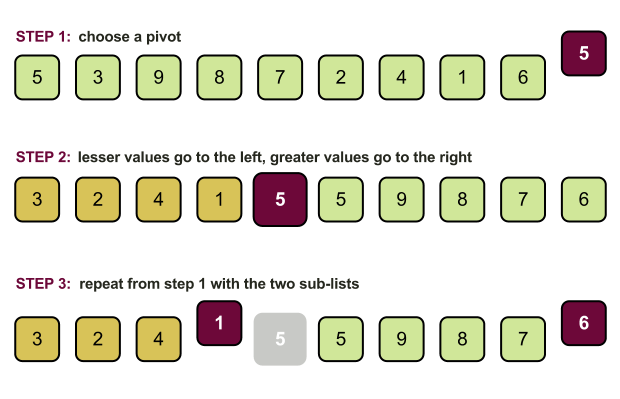
\includegraphics[scale=0.3]{img/quicksort_new.png}
\caption{Quicksort Algorithmus}
\end{figure}
Runtime: $O(n \cdot log(n))$
\end{frame}

\begin{frame}[fragile]
\frametitle{Quick Sort}
Worst Case: Array is already sorted.
\begin{figure}[h]
\centering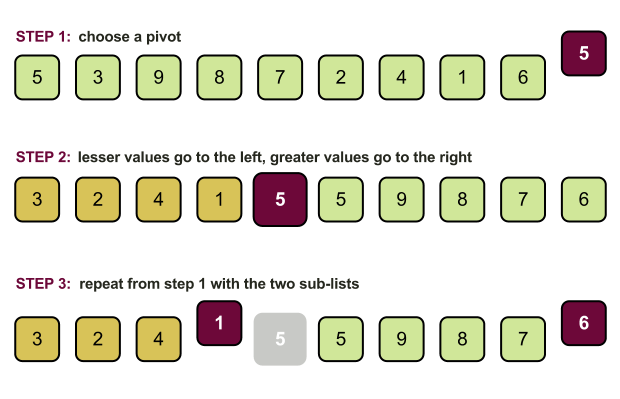
\includegraphics[scale=0.3]{img/quicksort_new.png}
\caption{Quicksort Algorithm Worst Case}
\end{figure}
Runtime: $O(n^2)$
\end{frame}

\begin{frame}[fragile]
\frametitle{Randomized Quick Sort}
Do not take the last element as pivot element, just choose
the pivot element randomly from all available elements.\\
Change the last element with the pivot element, therefore
the code developed before is still usable.
Runtime: $O(n \cdot log(n))$
\end{frame}

\begin{frame}[fragile]
\frametitle{Merge Sort}
\begin{figure}[h]
\centering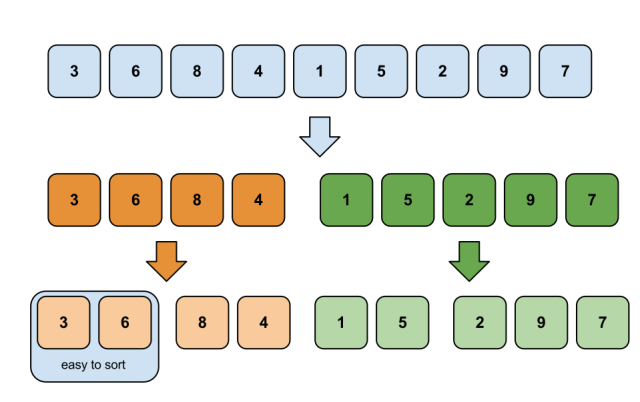
\includegraphics[scale=0.3]{img/mergesort_new.png}
\caption{Merge Sort Algorithm}
\end{figure}
Runtime: $O(n \cdot log(n))$
\end{frame}

\begin{frame}[fragile]
\frametitle{Performance}
Sorting of 100000 elements:
\begin{itemize}
\item Selection Sort: 9.27952s
\item Bubble Sort: 25.1975s
\item Quick Sort: 0.027657s
\item Merge Sort: 0.029053s
\item STL Sort: 0.009174s
\end{itemize}
\end{frame}


%\subsection{Searching}

\begin{frame}[fragile]
\frametitle{Searching}

The implementation of different searching algorithms should be based on
the abstract Search class as given in the following diagram:

\begin{figure}[h]
\centering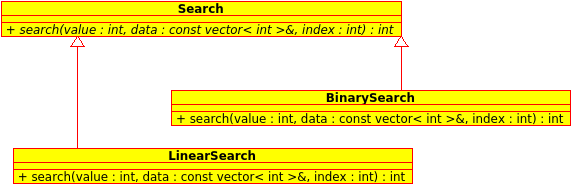
\includegraphics[scale=0.5]{img/search.png}
\caption{Searching Framework}
\end{figure}

\end{frame}

\begin{frame}[fragile]
\frametitle{Searching}
{\tiny
\lstinputlisting{code/search/search.h}
}

\end{frame}

\begin{frame}[fragile]
\frametitle{Linear Search}
Linear search is a method for finding a target value within a list.
It sequentially checks each element of the list for the target value until a match
is found or until all the elements have been searched.\\
\vspace{2mm}
Find 37\\
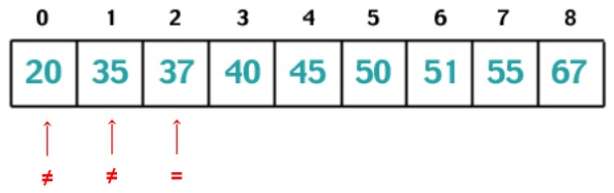
\includegraphics[scale=0.5]{img/linearsearch.png}\\
The result value is 2 (position where 37 is found)\\
\vspace{2mm}
Runtime: $O(n)$
\end{frame}

\begin{frame}[fragile]
\frametitle{Binary Search}
Binary search finds the position of a target value within a sorted array.
It compares the target value to the middle element of the array; if they are unequal,
the half in which the target cannot lie is eliminated and the search continues on the
remaining half until it is successful.\\
\vspace{2mm}
Find 37\\
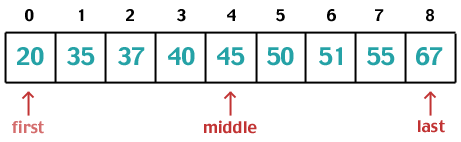
\includegraphics[scale=0.5]{img/binarysearch.png}\\
\vspace{2mm}
Runtime: $O(log(n))$
\end{frame}



%\subsection{Array}
\begin{frame}[fragile]
\frametitle{Array}
An array is stored as one piece in the memory.\\
Use an array if
\begin{itemize}
\item you need indexed or random access to elements
\item you know the number of elements which will be stored in the array
\item you need speed when iterating through all elements
\item memory is a concern (a linked list needs much more memory)
\end{itemize}
\end{frame}

\subsection{Linked List}
\begin{frame}[fragile]
\frametitle{Linked List}
In a linked list, all elements are distributed in the memory. An additional pointer
for each element is needed to store the location of the next element.\\
Use a linked list if
\begin{itemize}
\item you need constant time for insertions and deletions
\item you do not know how many elements will be stored in the list
\item you do not need random access
\end{itemize}
\end{frame}

\begin{frame}[fragile]
\frametitle{Linked List}
A linked list in the memory:\\
\vspace{1mm}
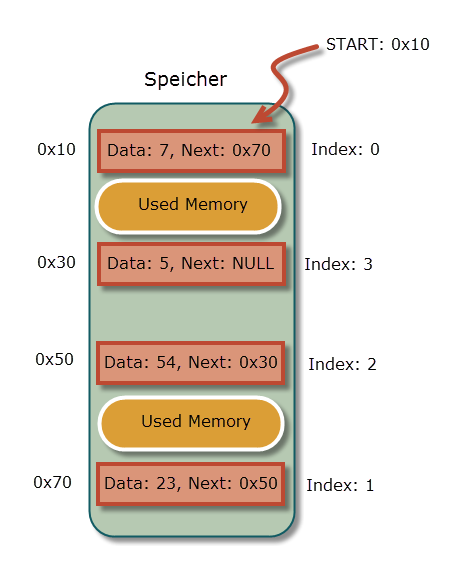
\includegraphics[scale=0.35]{img/linkedlist.png}
\end{frame}

\begin{frame}[fragile]
\frametitle{Linked List}
Insert into a linked list:\\
\vspace{1mm}
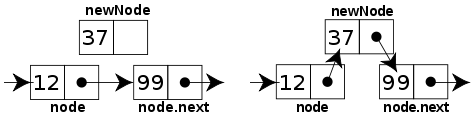
\includegraphics[scale=0.3]{img/linkedlist_insert2.png}\\
\vspace{5mm}
Delete from a linked list:\\
\vspace{1mm}
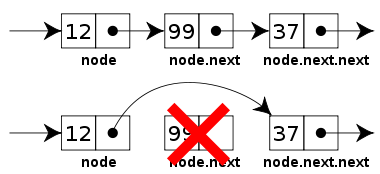
\includegraphics[scale=0.3]{img/linkedlist_remove2.png}
\end{frame}

\begin{frame}[fragile]
\frametitle{Array, Linked List}
\begin{exercise}
Create a abstract base class \verb|Container| which contains the most
important operations to read and write data into a container.
\end{exercise}
\begin{exercise}
Create 2 sub classes of the class \verb|Container|. Implement all abstract
methods (one class is based on an array, the other one on a linked list).
\end{exercise}
\end{frame}

\subsection{Stack}
\begin{frame}[fragile]
\frametitle{Stack}
A stack is a \emph{LIFO} (last in, first out) data type that serves as a collection
of elements with two principal operations: push and pop.\\
push adds an element to the collection, pop removes the last element that was added.\\
\vspace{1mm}
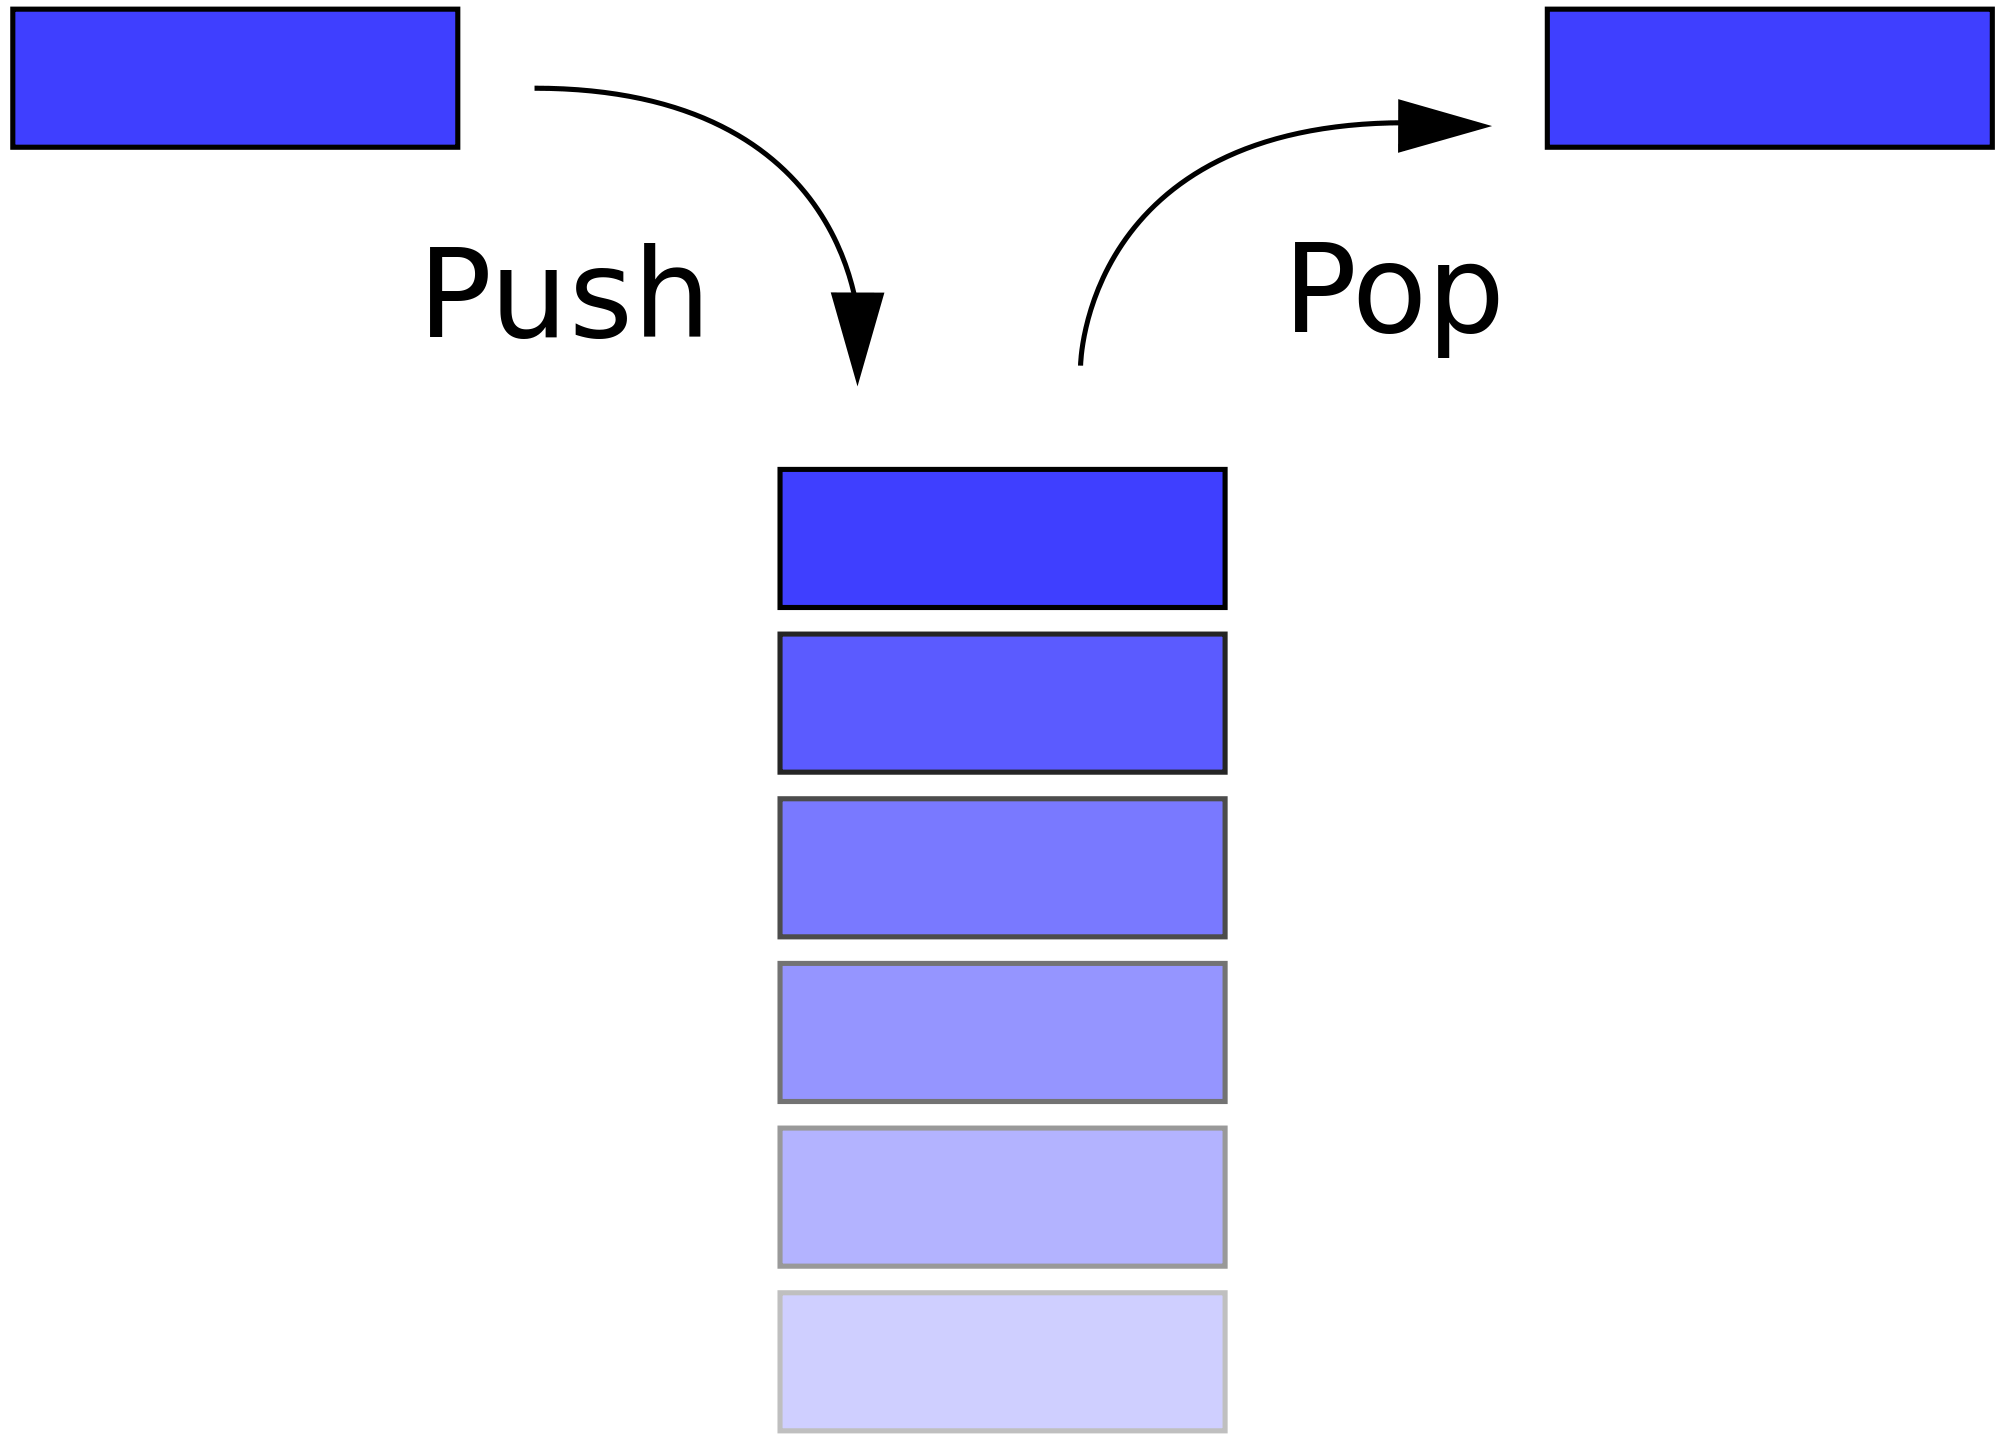
\includegraphics[scale=0.06]{img/stack.png}
\end{frame}

\begin{frame}[fragile]
\frametitle{Stack}
{\tiny
\begin{lstlisting}
class Stack {
private:
  int *values; // array based stack
  int maxNumberOfElement;
  int index;
private:
  Stack();
  Stack(const Stack & obj);
  Stack operator= (const Stack & obj);
  virtual ~Stack();
  bool pop(int & value);
  bool push(int value);
  bool top(int & value);
  int size();
  bool isEmpty();
};
\end{lstlisting}
}
\end{frame}

\subsection{Queue}
\begin{frame}[fragile]
\frametitle{Queue}
A queue is a \emph{FIFO} (first in, first out) data type that serves as a collection
of elements with two principal operations: enqueue and dequeue.\\
enque adds an element to the collection, deque removes the first element that was added.\\
\vspace{1mm}
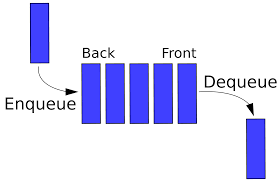
\includegraphics[scale=0.3]{img/queue.png}
\end{frame}

\begin{frame}[fragile]
\frametitle{Queue}
{\tiny
\begin{lstlisting}
class Queue {
private:
  Stack values; // stack based queue
private:
  Queue();
  Queue(const Stack & obj);
  Queue operator= (const Queue & obj);
  virtual ~Queue();
  bool deque(int & value);
  bool enque(int value);
  bool front(int & value);
  bool back(int & value);
  int size();
  bool isEmpty();
};
\end{lstlisting}
}
\end{frame}
%\subsection{String Matching}

\begin{frame}[fragile] 
  \frametitle{String Matching}
  String matching algorithms are an important class of string algorithms that try
  to find a place where one string (also called pattern) are found within a larger
  string or text.
  \vspace{3mm}
  \begin{itemize}
  \item Naive
  \item Boyer Moore
  \end{itemize}
\end{frame}

\begin{frame}[fragile] 
  \frametitle{Naive}
  Align the pattern at the beginning of the text and compare each character.
  Move the character one position to the right in case of a mismatch!\\
  \vspace{3mm}
  {\small
  \verb|T: HERE IS A SIMPLE EXAMPLE|\\
  \verb|P: EXAMPLE|\\
  \verb|    EXAMPLE|\\
  \verb|     EXAMPLE|\\
  \verb|      EXAMPLE|\\
  \verb|       EXAMPLE|\\
  \verb|        ...|\\
  \verb|                    EXAMPLE|\\
  }
\end{frame}

\begin{frame}[fragile] 
\frametitle{Naive - Exercise}
\begin{exercise}
Implement the Naive algorithm.
\begin{lstlisting}
int Naive::bm(
  const string & text, const string & pattern)
\end{lstlisting}
\end{exercise}
\end{frame}

\begin{frame}[fragile] 
  \frametitle{Boyer Moore}
  This algorithm will use the knowledge from the character comparisons to skip
  future alignments that will definitly not match.\\
  {\bf Start to scan the pattern from the right side!}\\
  In case of a mismatch we can skip comparisons in case the character in the text
  doesn’t happen to appear in the pattern.
\end{frame}

\begin{frame}[fragile]
  \frametitle{Boyer Moore}
  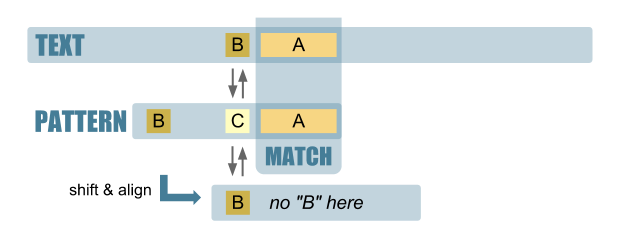
\includegraphics[scale=0.4]{img/bm1.png}\\
  \vspace{1mm}
  The mismatched character B from the text appears in the beginning of the pattern.
  Therefore the pattern will be shifted to the right until character B in the
  pattern and text are aligend.
\end{frame}

\begin{frame}[fragile]
  \frametitle{Boyer Moore}
  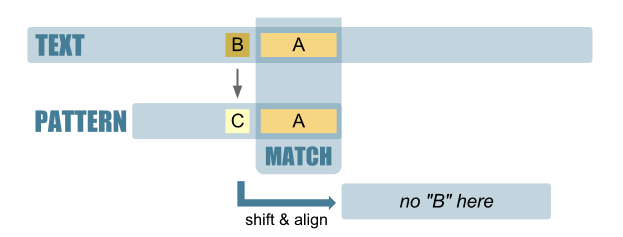
\includegraphics[scale=0.4]{img/bm2.png}\\
  \vspace{1mm}
  If the mismatched character B is not contained in the pattern, then the whole
  pattern can be shifted forward.
\end{frame}

\begin{frame}[fragile] 
\frametitle{Boyer Moore - Example}
\verb|T: HERE IS A SIMPLE EXAMPLE|\\
\verb|P: EXAMPLE|\\
\verb|          EXAMPLE|\\
\verb|            EXAMPLE|\\
\verb|               EXAMPLE|\\
\verb|                    EXAMPLE|
\end{frame}

\begin{frame}[fragile] 
\frametitle{Boyer Moore}
The shift offset will be precalculated. In case of a mismatch there is a table to
look up the shift offset.\\

\begin{tabular}{l|l}
A & 5\\
B & 7 (Pattern length)\\
C & 7\\
...& ...\\
X & 6\\
Y & 7\\
Z & 7
\end{tabular}
\end{frame}

\begin{frame}[fragile] 
\frametitle{Boyer Moore - Exercise}
\begin{exercise}
Implement the Boyer Moore algorithm.
\begin{lstlisting}
int StringUtil::bm(
  const string & text, const string & pattern)
\end{lstlisting}
\end{exercise}
\begin{exercise}
Create a meaningful testcase and compare the performance between the naive and Boyer Moore algorithm. 
\end{exercise}
\end{frame}

\begin{frame}[fragile]
\frametitle{Edit Distance}
The edit distance is a way of quantifying how dissimilar two strings are to one another by counting the minimum number of operations (insert, delete, substitue) required to transform one string into the other.\\
\vspace{3mm}
If a user types \emph{graffe}? What could he mean?
\begin{itemize}
\item graf
\item graft
\item grail
\item giraffe
\end{itemize}

\end{frame}

\begin{frame}[fragile]
\frametitle{Edit Distance - Example}
\verb|I N T E * N T I O N|\\
\verb|' ' ' ' ' ' ' ' ' '|\\
\verb|* E X E C U T I O N|\\
 
\vspace{3mm}

The editing distance is 5.\\
3 Substitutions + 2 Insertions\\

\vspace{3mm}

\begin{exercise}
What is the minimum editing distance of \emph{GUMBO} and \emph{GAMBOL}?
\end{exercise}

\end{frame}

\begin{frame}[fragile]
\frametitle{Edit Distance}
Two string s and t are given.\\
$m = length(s)$\\
$n = length(t)$\\
\vspace{3mm}
Initialize\\
$D_{0,0} = 0$\\
$D_{i,0} = i, 1 \leq i \leq m$\\
$D_{0,j} = j, 1 \leq j \leq n$
\end{frame}

\begin{frame}[fragile]
\frametitle{Edit Distance}
\begin{tabular}{|c|c|c|c|c|c|c|}
\hline
 & & G & U & M & B & O\\
\hline
 & 0 & 1 & 2 & 3 & 4 & 5\\
\hline
G & 1 & & & & &\\
\hline
A & 2 & & & & &\\
\hline
M & 3 & & & & &\\
\hline
B & 4 & & & & &\\
\hline
O & 5 & & & & &\\
\hline
L & 6 & & & & &\\
\hline
\end{tabular}
\end{frame}

\begin{frame}[fragile]
\frametitle{Edit Distance}
Calculate each cell with the following formula:
\begin{align}
D_{i,j}= min \left\{
\begin{aligned} & D_{i-1,j-1} + 0 & & t_i = s_i\\
& D_{i-1,j-1} + 1 & & t_i \neq s_i (Substitute)\\
& D_{i,j-1} + 1 & & (Insert)\\
& D_{i-1,j} + 1 & & (Delete)\\
\end{aligned}\right.
\end{align}
\end{frame}

\begin{frame}[fragile]
\frametitle{Edit Distance}
\begin{tabular}{|c|c|c|c|c|c|c|}
\hline
 & & G & U & M & B & O\\
\hline
 & 0 & 1 & 2 & 3 & 4 & 5\\
\hline
G & 1 & 0 & 1 & 2 & 3 & 4\\
\hline
A & 2 & 1 & 1 & 2 & 3 & 4\\
\hline
M & 3 & 2 & 2 & 1 & 2 & 3\\
\hline
B & 4 & 3 & 3 & 2 & 1 & 2\\
\hline
O & 5 & 4 & 4 & 3 & 2 & 1\\
\hline
L & 6 & 5 & 5 & 4 & 3 & {\bf 2}\\
\hline
\end{tabular}\\
\vspace{3mm}
The final result is in the lower right hand corner!
\end{frame}


\section{Programming with QT}

\frame
{
\frametitle{What is QT?}
\begin{itemize}
\item Company History: Trolltech (1994-2008), Nokia (2008-2012), Digia (2012-2014), The QT Company (2014-)
\item QT is a cross-platform application and UI framework
\item QT provides intuitive C++ class libraries
\item Current Version: 5.10.0 (7-DEC-2017)
{\tiny
\begin{itemize}
\item 3D Graphics with OpenGL
\item Multithreading
\item Network Connectivity
\item ...
\end{itemize}
}
\item QT provides portability across several platforms\\
\begin{itemize}
\item Windows
\item OSX
\item Unix/Linux
\item Android
\item ...
\end{itemize}
\item QT provides development tools (IDE)
\end{itemize}
}

\subsection{QT Development Environment}
\frame
{
\frametitle{QT Development Environment}
Requirements
\begin{itemize}
\item MinGW
\item QT SDK
\item Editor: Notepad++, emacs, Ultra Edit, Atom, ...
\end{itemize}
\vspace{5mm}
Development Environment
\begin{itemize}
\item Console
\item QT Creator
\item Visual Studio, Code Blocks, ... (not supported@hf-ict)
\end{itemize}
}

\frame
{
\frametitle{Development with Console}
\begin{itemize}
\item Change to the directory containing the source code
\item Type \emph{qmake -project [CONFIG+=console]}
\item Type \emph{qmake}
\item Type \emph{mingw32-make}
\end{itemize}

Ensure that the correct Environment variables are set (PATH)!\\
\begin{itemize}
\item QT bin folder
\item MINGW bin folder
\end{itemize}
}

\frame
{
\frametitle{Development with QT Creator}
\begin{itemize}
\item Start the QT Creator application
\item File - New - QT 5 Gui Application
\item Enter project name
\item Select required modules
\item Start the application with Build - Run
\end{itemize}
}

\frame
{
\frametitle{Development with QT Creator}
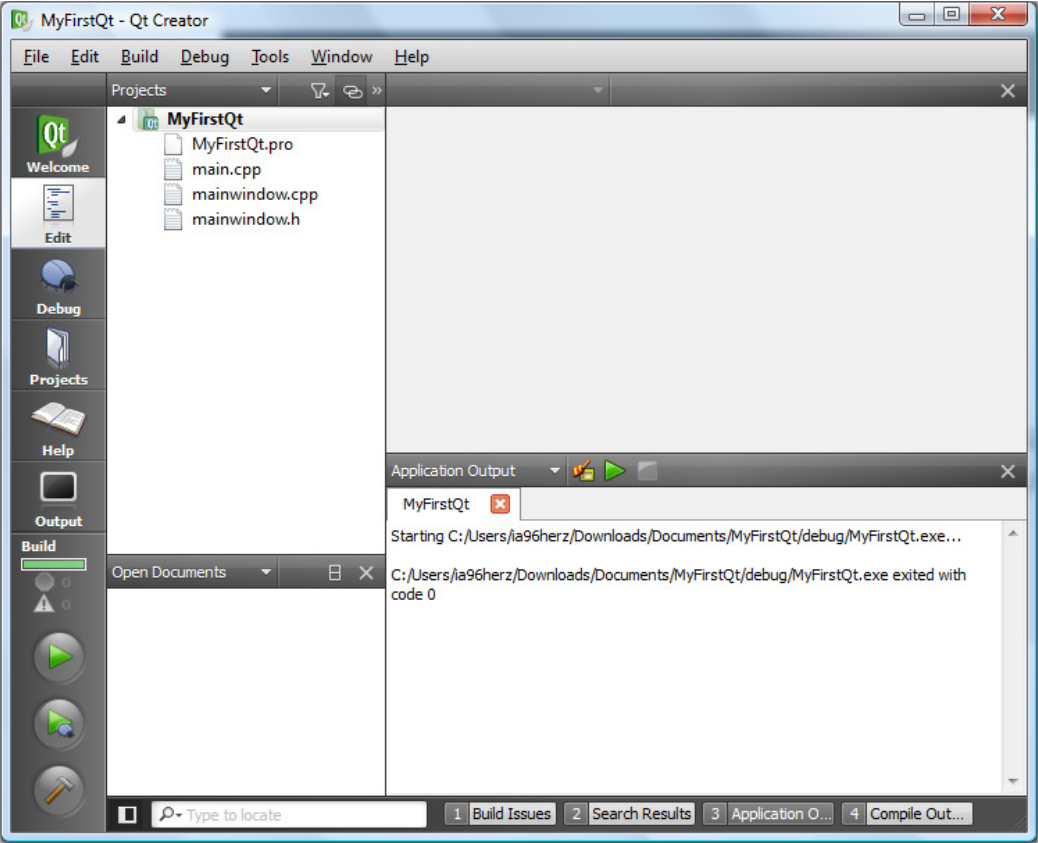
\includegraphics[width=250pt]{img/qtcreator.png}
}

\frame
{
\frametitle{Resources}
The complete Documentation, API and Examples can be found at
\begin{itemize}
\item https://doc.qt.io
\end{itemize}
Books:
\begin{itemize}
\item Mastering Qt 5\\
Guillaume Lazar, Robin Penea\\
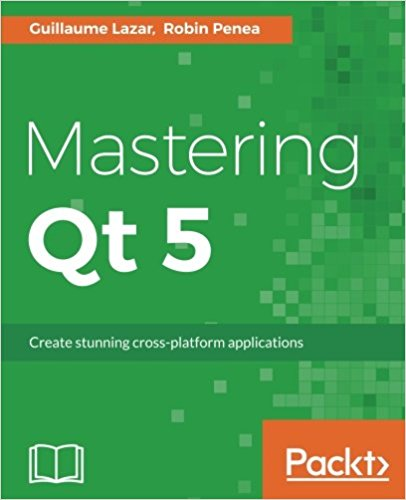
\includegraphics[width=90pt]{img/qt5book.jpg}
\end{itemize}
}

\frame
{
\frametitle{QT - HF-ICT}
\begin{itemize}
\item Introduction
\item Small Projects (QT Basics, Layouts, Slots, ...)
\item Fractals (QT Painting)
\item Game (Multithreading)
\end{itemize}
}

\subsection{Hello World - Hello QT - Basics}
\frame
{
\frametitle{Hello QT - My first QT program}
\lstinputlisting{code/qt/helloqt/helloqt.cpp}
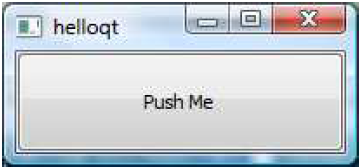
\includegraphics[width=85pt]{img/helloqt.png}
}

\frame
{
\frametitle{Exercise - Hello QT}
\begin{exercise}
\begin{itemize}
\item Setup your QT development environment
\item Write a \emph{Hello QT} application
\end{itemize}
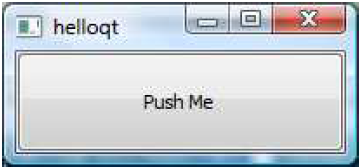
\includegraphics[width=85pt]{img/helloqt.png}
\end{exercise}
}

\begin{frame}[fragile]
\frametitle{QWidget}
Every gui element (single element or a group of element) in QT is a Widget (Window Gadget).
\vspace{5mm}
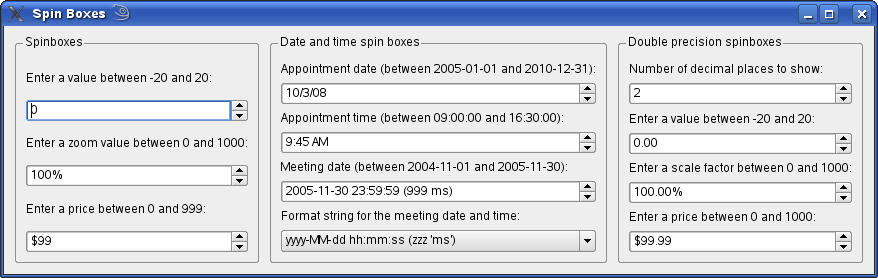
\includegraphics[width=280pt]{img/widget.png}
\end{frame}

\begin{frame}[fragile]
\frametitle{Exercise - QT Standard Widgets}
\begin{exercise}
Create the following three QT applications:\\
\vspace{5mm}
\\
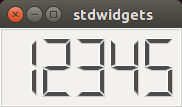
\includegraphics[width=75pt]{code/qt/stdwidgets/w1.png}
\hspace{5mm}
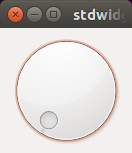
\includegraphics[width=50pt]{code/qt/stdwidgets/w2.png}
\hspace{5mm}

\includegraphics[width=100pt]{code/qt/stdwidgets/w3.png}
\end{exercise}
\end{frame}

\begin{frame}[fragile]
\frametitle{Exercise - 2 Widgets in one Window}
\begin{exercise}
Can you display two widgets in one window?\\
\vspace{5mm}
\\
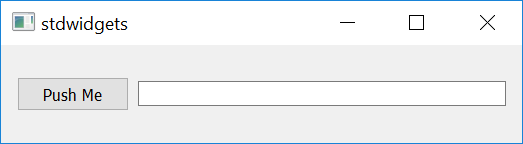
\includegraphics[width=120pt]{code/qt/stdwidgets/w4.png}
\end{exercise}
\end{frame}


\begin{frame}[fragile]
\frametitle{QDebug vs cout}
\begin{itemize}
\item qDebug()
\item qInfo()
\item qWarning()
\item qCritical()
\item qFatal()
\end{itemize}

\begin{lstlisting}
qDebug() << "some debug output...";
\end{lstlisting}

Switch off debug output:
\begin{lstlisting}
qmake -project DEFINES+=QT_NO_DEBUG_OUTPUT
\end{lstlisting}

\end{frame}


\subsection{Layout Manager}
\frame
{
\frametitle{Layout Manager}
The following Layout Managers are available in QT:
\begin{itemize}
\item QHBoxLayout
\item QVBoxLayout
\item QGridLayout
\item QFormLayout
\item Null Layout
\item ...
\end{itemize}
}

\begin{frame}[fragile]
\frametitle{QHBoxLayout (QVBoxLayout)}
Horizontal arrangement of all widgets.\\
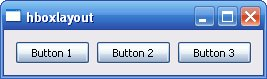
\includegraphics[width=112pt]{code/qt/hbox/hboxlayout.jpg}\\
{\tiny
\lstinputlisting{code/qt/hbox/hbox.cpp}
}
\end{frame}

\begin{frame}[fragile]
\frametitle{QHBoxLayout (QVBoxLayout)}
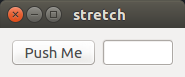
\includegraphics[width=100pt]{code/qt/stretch/stretch1.png}\\
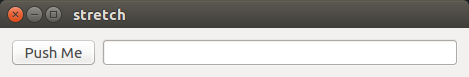
\includegraphics[width=150pt]{code/qt/stretch/stretch2.png}\\
\begin{lstlisting}
button->sizePolicy().expandingDirections();
// QFlags()
input->sizePolicy().expandingDirections();
// QFlags(0x1)
// 0x1: Qt::Horizontal
\end{lstlisting}
\end{frame}

\frame
{
\frametitle{QGridLayout}
Arrangement of all widgets in a grid.\\
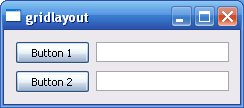
\includegraphics[width=100pt]{code/qt/grid/gridlayout.jpg}\\
{\tiny
\lstinputlisting{code/qt/grid/gridlayout.cpp}
}
}

\frame
{
\frametitle{QFormLayout}
The QFormLayout class manages forms of input widgets and their associated labels.\\
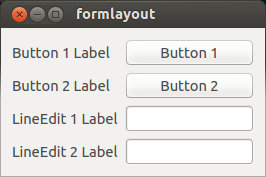
\includegraphics[width=100pt]{img/formlayout.png}\\
{\tiny
\lstinputlisting{code/qt/formlayout/mywidget.cpp}
}
}

\frame
{
\frametitle{Null Layout}
No layout manager\\
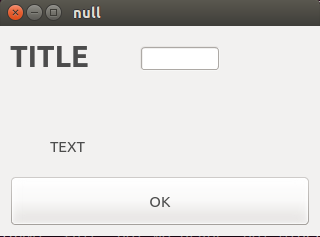
\includegraphics[width=72pt]{code/qt/null/xylayout.png}\\
{\tiny
\lstinputlisting{code/qt/null/mywidget.cpp}
}
}

\begin{frame}[fragile]
\frametitle{Modular Programming}
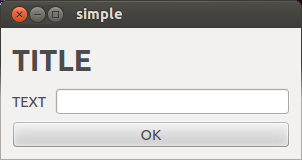
\includegraphics[width=140pt]{img/simple.png}
\hspace{4mm}
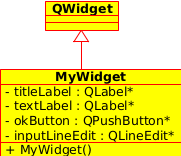
\includegraphics[width=100pt]{img/simplecd.png}
\end{frame}

\begin{frame}[fragile]
\frametitle{Modular Programming}
{\tiny
\lstinputlisting{code/qt/simple/mywidget.h}
}
\end{frame}

\begin{frame}[fragile]
\frametitle{Modular Programming}
{\tiny
\lstinputlisting{code/qt/simple/mywidget.cpp}
}
\end{frame}

\begin{frame}[fragile]
	\frametitle{Modular Programming}
	{\tiny
	\lstinputlisting{code/qt/simple/main.cpp}
	}
\end{frame}

\frame
{
	\frametitle{QMainWindow}
	A main window provides a framework for building an application's user interface.
	Qt has QMainWindow and its related classes for main window management.
	QMainWindow has its own layout to which you can add QToolBars, QDockWidgets,
	a QMenuBar, and a QStatusBar. The layout has a center area that can be occupied
	by any kind of widget.\\
	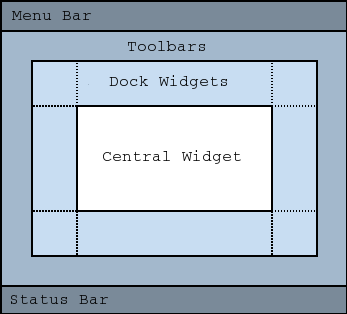
\includegraphics[width=140pt]{img/mainwindowlayout.png}

}

\frame
{
	\frametitle{Change Background Color of QLineEdit}
	\lstinputlisting{code/qt/color.cpp}
}

\frame
{
	\frametitle{Validate Input}
	There are two ways on how to validate the input values.
	\begin{itemize}
	\item Using a validator
	{\tiny
	\lstinputlisting{code/qt/validator/method1.cpp}
	}
	\item Check the values after commit
	{\tiny
	\lstinputlisting{code/qt/validator/method2.cpp}
	}
	\end{itemize}
}


\subsection{Event Handling}
\frame
{
	\frametitle{Slots}
	Every widget may fire events (Signals). These events can be catched be a method
	called slot.\\
	Take a look on the API to check which Signal and Slots are available for each
	widget.\\
	Example: Signals of the class QPushButton:
	\begin{itemize}
	\item clicked(bool checked=false)
	\item pressed()
	\item released()
	\item toggled(bool checked)
	\end{itemize}
}

\frame
{
	\frametitle{Slots}
	A class which implements a slot must
	\begin{itemize}
	\item be inherited from the class QObject (or a subclass)
	\item contain the Q\textunderscore OBJECT statement
	\item contain the public slots section
	\end{itemize}
	\lstinputlisting{code/qt/slot.cpp}
}

\frame
{
	\frametitle{Slots}
	Within the code, the Signal and Slot must be connected.
	\lstinputlisting{code/qt/connection.cpp}
	The senderObject fires the event (signal). The receiverObject contains the slot.
}

\begin{frame}[fragile]
	\frametitle{My first slot}
	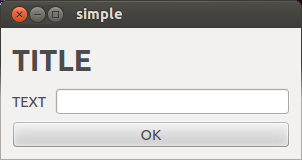
\includegraphics[width=140pt]{img/simple.png}
	\hspace{4mm}
	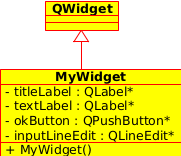
\includegraphics[width=100pt]{img/simplecd.png}\\
	\vspace{3mm}
	Add a simple slot called \verb|onButtonClicked| in the class \verb|MyWidget|.
\end{frame}

\begin{frame}[fragile]
	\frametitle{My first slot}
	\begin{lstlisting}
class MyWidget : public QWidget {
Q_OBJECT
private:
  ... // see slide before
public:
  ... // see slide before
public slots:
  void onButtonClicked();
	\end{lstlisting}
\end{frame}

\begin{frame}[fragile]
	\frametitle{My first slot}
	\begin{lstlisting}
MyWidget::MyWidget() {
  ... // see slide before
  QOBject::connect(
    okButton, SIGNAL(clicked()),
    this, SLOT(onButtonClicked()));
}

void MyWidget::onButtonClicked() {
  // delete the content of the QLineEdit component
  inputLineEdit->clear();
}
	\end{lstlisting}
\end{frame}

\begin{frame}[fragile]
	\frametitle{Exercise - Event Handling}
	Take the code from the example above. Add a new class called \verb|EventHandler|
	and move the slot \verb|onButtonClicked| from the class \verb|MyWidget| to the
	class \verb|EventHandler|. The functionality should still be the same.
\end{frame}

\begin{frame}[fragile]
	\frametitle{Exercise - Event Handling}
	The major difficulties in this exercise are:
	\begin{itemize}
	\item A new object of the class \verb|EventHandler| must be created and used
	within the \verb|QObject::connect| statement.
	\item A way must be found to access the \verb|inputLineEdit| component, which
	is now in another class than the slot.
	\end{itemize}
\end{frame}

\begin{frame}[fragile]
\frametitle{Signals}
Every widget may fire events (Signals). A signal will be implemented
in the following way:

{\small
\begin{lstlisting}
class MyClass : public QObject {
public:
  MyClass();
  ...
  void someMethod();
signals:
  void somethingHappens();
};
\end{lstlisting}
}
A signal method has no implementation. The signal itself can be
triggered by calling the method:

{\small
\begin{lstlisting}
void MyClass::someMethod() {
   emit somethingHappens();
}
\end{lstlisting}
}

\end{frame}

\subsection{Dialogs}
\begin{frame}[fragile]
\frametitle{Dialogs}
In a graphical user interface, a dialog is a window used to enable communication between
a computer and the user. It may communicate information to the user, prompt the user for
a response, or both. A dialog can be displayed in modal mode.\\
\vspace{3mm}
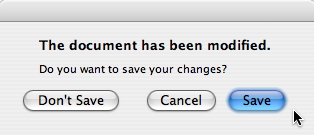
\includegraphics[width=160pt]{img/dialog1.png} 
\end{frame}

\begin{frame}[fragile]
\frametitle{Dialogs}
The class QMessageBox could be used fo standard dialogs:
\vspace{3mm}
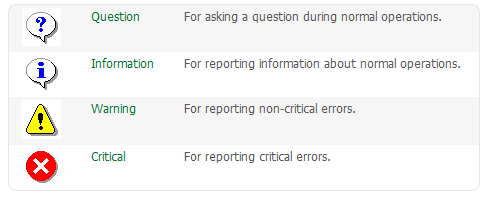
\includegraphics[width=200pt]{img/messagebox.png}
{\tiny
\begin{lstlisting}
int result = QMessageBox::warning( // warning, critical, ...
  this, // parent
  "TITLE",
  "TEXT",
  QMessageBox::Save | QMessageBox::Discard | QMessageBox::Cancel
);
\end{lstlisting}
}
\end{frame}

\begin{frame}[fragile]
\frametitle{Dialogs}
If a custom dialog is needed, create a class inherited from QDialog.
A dialog is created like a QWidget (actually it is a QWidget) with
some additional important dialog functionality.
\begin{itemize}
\item Modal - Calling window is disabled and the dialog is always in foreground.
\item Result - A dialog normally provides a result value.
(e.g. Ok, Cancel Button Clicked)
\end{itemize}
\end{frame}

\begin{frame}[fragile]
	\frametitle{Exercise - Modular Programming}
	\begin{exercise}
  Implement a gui to validate a credit card number (only the number).\\
  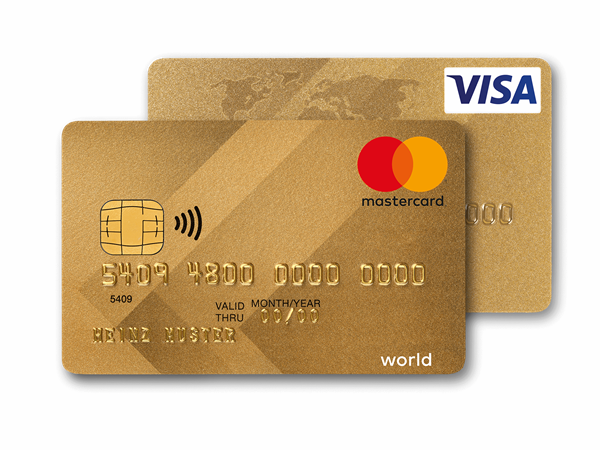
\includegraphics[width=140pt]{img/creditcard.png}\\
  The Luhn formula can be used to validate the number.
	\end{exercise}
\end{frame}


\subsection{Painting}
\begin{frame}[fragile]
\frametitle{Painting}
To paint something on a QT Widget, the method paintEvent must be overwritten:
\lstinputlisting{code/qt/paint/paint.cpp}
\end{frame}

\begin{frame}[fragile]
\frametitle{Painting}
The QPainter objects supports many method to draw specific geometric figures:
	(e.g. Arc, Line, Point)\\
	\vspace{3mm}
        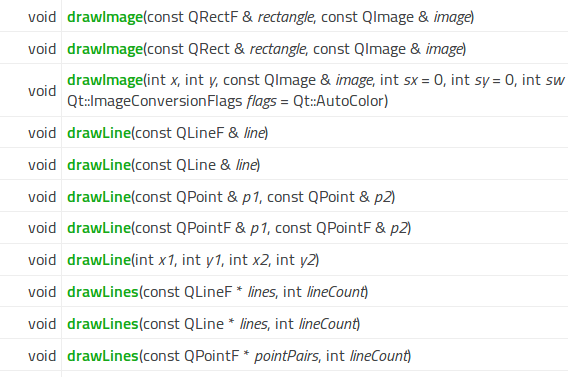
\includegraphics[width=190pt]{img/painter.png}
\end{frame}

\begin{frame}[fragile]
\frametitle{Exercise - Moiree}
Create an application which draws the following picture:
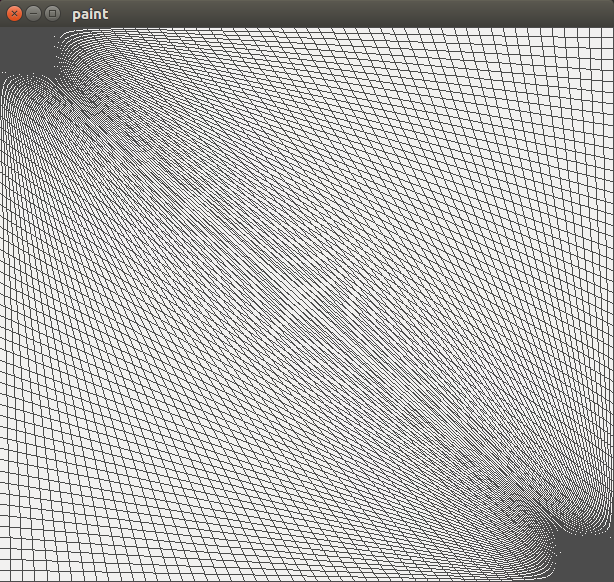
\includegraphics[width=190pt]{img/moiree.png}
\end{frame}

\begin{frame}[fragile]
\frametitle{Exercise - Sierpinski}
Draw on a widget with the following algorithm:
{\small
\begin{enumerate}
\item Create 3 random points A, B and C. Preferably the 3 points should
be a triangle stretched over the widget.
\item Define a point (x,y) which is equal to point A.
\item Define randomly a point A, B or C. This point is called Z.
\item Calculate the middlepoint ($x_m$ and $y_m$) between Z and (x, y).
\item Draw a point at position $x_m$ and $y_m$.
\item Set $x=x_m$ and $y=y_m$.
\item o to step 3
\end{enumerate}
}
Draw about 100000 points. In addition colors could also be used at step 3. In case of point A (green), B (blue) and C (red).
\end{frame}

\subsection{Mouse Events}
\begin{frame}[fragile]
\frametitle{Mouse Events}
Mouse move and and mouse click events can be tracked on a widget by
overwritting one (or both) of the following methods:

\begin{itemize}
\item \verb|mouseMoveEvent(QMouseEvent *event)|\\
Do not forget to switch on mouse tracking (\verb|setMouseTracking(true)|) to handle these events.
\item \verb|mousePressEvent(QMouseEvent *event)|
\item \verb|mouseDoubleClickEvent(QMouseEvent *event)|
\item \verb|mouseReleaseEvent(QMouseEvent *event)|
\end{itemize}

\end{frame}

\subsection{Threads}
\begin{frame}[fragile]
\frametitle{Threads}
A Thread in QT may be implemented in the following way:
{\tiny
\begin{lstlisting}
class MyThread : public QThread {
public:
  void run();
};

void MyThread::run() {
  // code which will be executed in the thread
}

// creating a thread
MyThread *mt = new MyThread();
// starting a thread
mt.start();
\end{lstlisting}
}
\end{frame}

\begin{frame}[fragile]
\frametitle{Threads}
Endless Thread with the possibility to stop.
{\tiny
\begin{lstlisting}
class MyThread : public QThread {
private:
  bool running;
public:
  MyThread();
  void stopThread();
  void run();
};

MyThread::MyThread() : running(true) {}

void MyThread::stopThread() {
  running = false;
}

void MyThread::run() {
  while(running) {
  // code which will be executed in the thread
  msleep(50);
  }
}
\end{lstlisting}
}
\end{frame}

\begin{frame}[fragile]
\frametitle{Threads}
Thread Synchronization - Producer Consumer\\
{\tiny
The Producer-Consumer problem describes two processes, the producer and the consumer, who share a data container. The producer's job is to generate data. The consumer's job is to consume (and remove) the data. The problem is to make sure that the producer won't try to add data into the container if it's full and that the consumer won't try to consume data from an empty container.
}
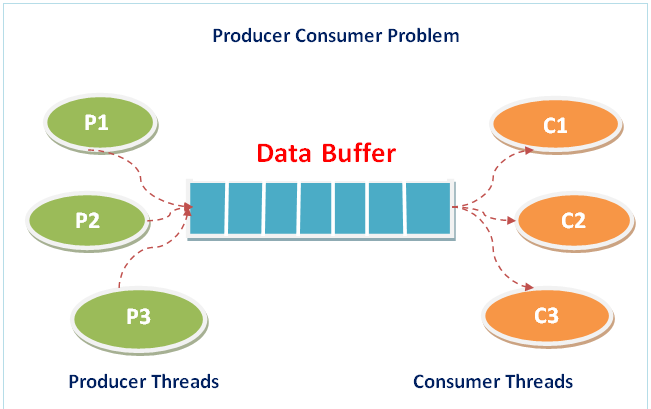
\includegraphics[width=190pt]{img/prodcon.png}

\end{frame}

\begin{frame}[fragile]
\frametitle{Threads}
Thread Synchronization - Producer Consumer\\
QT provides several classes for thread synchronization:
\begin{itemize}
\item QMutex
\item QSemaphore
\item QMutexLocker
\item QWaitConditon
\item QReadWriteLock
\end{itemize}

\end{frame}

\begin{frame}[fragile]
\frametitle{Threads}
Thread Synchronization - Producer Consumer\\
{\tiny
\lstinputlisting{code/qt/thread/prodcon.cpp}
}

\end{frame}

\begin{frame}[fragile]
\frametitle{QT Game}
The following slides will describe how to create a simple game in QT.
\begin{itemize}
\item Idea
\item Gui Design
\item Game Objects
\item Game Thread
\item Collision Detection
\item Sound
\end{itemize}
\end{frame}

\begin{frame}[fragile]
\frametitle{QT Game}
Gui Design
\begin{itemize}
\item MainWindow
\item MainWidget
\item GameArea
\end{itemize}
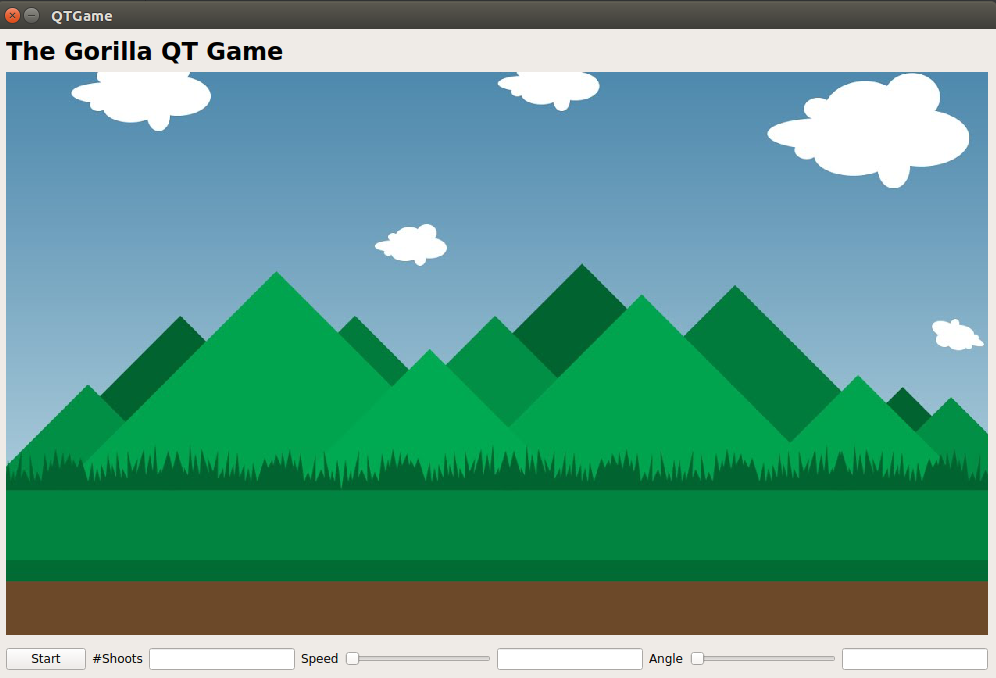
\includegraphics[width=220pt]{img/qtgamegui.png}
\end{frame}

\begin{frame}[fragile]
\frametitle{QT Game}
Gui Design - Class Diagram
\includegraphics[width=220pt]{img/qtgame_cdgui.png}
\end{frame}

\begin{frame}[fragile]
\frametitle{QT Game}
Game Objects
\begin{itemize}
\item GameObject (abstract base class)
\item Player
\item Obstacle
\item Shoot
\end{itemize}
\includegraphics[width=220pt]{img/qtgame_cdgo.png}
\end{frame}

\begin{frame}[fragile]
\frametitle{QT Game}
Shoot - Projectile motion\\
\includegraphics[width=100pt]{img/pro_motion.png}

{\small
\begin{lstlisting}
const double g = 9.81;
double rad = 3.1415926 / 180 * angle;
int dx = speed/3 * cos(rad) * t;
int dy = speed/3 * sin(rad) * t - (g/2) * pow(t,2);
t = t+0.1;
x = x + dx/2;
y = y - dy/2;
\end{lstlisting}
}
\end{frame}

\begin{frame}[fragile]
\frametitle{QT Game}
Thread
\begin{itemize}
\item Thread
\end{itemize}
\includegraphics[width=100pt]{img/qtgame_cdthread.png}
\end{frame}

\begin{frame}[fragile]
\frametitle{QT Game}
Collision Detection
\begin{itemize}
\item CollisionDetection
\end{itemize}
\includegraphics[width=220pt]{img/qtgame_cdcd.png}
\end{frame}

\begin{frame}[fragile]
\frametitle{QT Game}
Your additional tasks
\begin{itemize}
\item Rotating banana
\item Remove game objects if they are out of bounds
\item Include sound
\end{itemize}
\end{frame}


%\subsection{Database Access}
%\begin{frame}[fragile]
%\end{frame}
%\subsection{Network Connections}
%\begin{frame}[fragile]
%\end{frame}


%\section{Latex Samples}
\begin{frame}[fragile]
  \frametitle{Latex Samples}
  \begin{itemize}
  \item Bilder (png)
  \item Code Fragmente
  \item Übungen
  \item Theorem
  \item Example
  \end{itemize}
\end{frame}

\begin{frame}[fragile]
  \frametitle{Bilder (png)}
  \centering\includegraphics[scale=0.4]{quicksort.png}
\end{frame}

\begin{frame}[fragile]
  \frametitle{Code Fragmente}
  \begin{lstlisting}
  // my first program in C++
  \end{lstlisting}
  \emph{Dies ist eine Kommentar Zeile. Alle Zeilen die mit // beginnen sind
  Kommentare und haben keine Auswirkung auf das Programm. Sie werden
  genutzt um den Code mit Erkl"arungen zu erg"anzen.}
  \vspace{3mm}
  \emph{In C++ existieren zwei M"oglichkeiten f"ur Kommentare:}
  \begin{lstlisting}
  // Dieser Kommentar geht bis ans Ende der Zeile
  /* Dieser Kommentar endet
  beim Erscheinen der Zeichenfolge */
  \end{lstlisting}
\end{frame}

\begin{frame}[fragile]
  \frametitle{Übungen}
  \begin{exercise}
  Das ist eine Übung...
  \end{exercise}
\end{frame}

\begin{frame}[fragile]
  \frametitle{Theorem}
  \begin{theorem}
  Das ist ein Theorem...
  \end{theorem}
\end{frame}

\begin{frame}[fragile]
  \frametitle{Example}
  \begin{example}
  Das ist ein Beispiel...
  \end{example}
\end{frame}


\end{document}
